\documentclass[12pt]{article}

%\usepackage{mathptm}  
\usepackage{a4}
\usepackage{hyperref}
\usepackage{color}
\usepackage{graphicx}
\usepackage{fancyhdr}
\usepackage{multicol}
\usepackage{amstext}
\usepackage{amsmath}
%\usepackage{fullpage}
%\usepackage{parskip}
\usepackage[colon]{natbib}
%\usepackage{rotating}
\usepackage{pdflscape}
\usepackage{longtable}
\usepackage{caption}
\usepackage{subcaption}
%\usepackage[nomarkers,figuresonly]{endfloat}
\usepackage{amsfonts}
\usepackage{pifont}
\usepackage{authblk}
\usepackage{epstopdf}
\usepackage{multirow}
\usepackage{amsfonts}
\usepackage{bigints}
\usepackage{verbatim}

\textwidth 160mm
\textheight 235mm
\oddsidemargin 0mm
\topmargin -15mm
\baselineskip 13pt
\parskip 1pc
\parindent 0pc

\pagestyle{fancy}
\cfoot{\thepage}

\renewcommand{\headrulewidth}{0.2pt}
\renewcommand{\footrulewidth}{0.2pt}

\newcommand\Rey{\mbox{\textit{Re}}}  % Reynolds number
\newcommand\Bo{\mbox{\textit{Bo}}}  % Bond number
\newcommand\Ca{\mbox{\textit{Ca}}} %Capillary number

\definecolor{darkred}{rgb}{0.80,0.00,0.05}
\definecolor{blue}{rgb}{0.00,0.00,0.95}
\definecolor{darkgreen}{rgb}{0.00,0.60,0.0}
\definecolor{gray}{rgb}{0.95,0.9,0.9}

\usepackage{listings}
\lstset{language=C++}
\lstset{backgroundcolor=\color{gray}}
\lstset{breaklines=true}
\lstset{basicstyle=\ttfamily\small}
\lstset{showstringspaces=false}
\lstset{keywordstyle=\color{blue}\bfseries}
\lstset{commentstyle=\ttfamily\small\color{darkgreen}}
\lstset{identifierstyle=\color{darkred}\bfseries}
\lstset{numbers=left,numberstyle=\tiny}
\lstset{columns=fixed,basewidth=0.45em}

\DeclareMathOperator\erf{erf}

\linespread{1.5}

\def\Xint#1{\mathchoice
{\XXint\displaystyle\textstyle{#1}}%
{\XXint\textstyle\scriptstyle{#1}}%
{\XXint\scriptstyle\scriptscriptstyle{#1}}%
{\XXint\scriptscriptstyle\scriptscriptstyle{#1}}%
\!\int}
\def\XXint#1#2#3{{\setbox0=\hbox{$#1{#2#3}{\int}$}
\vcenter{\hbox{$#2#3$}}\kern-.5\wd0}}
\def\ddashint{\Xint=}
\def\dashint{\Xint-}


\begin{document}
\thispagestyle{empty}

\title{Low Reynolds number gravitational settling of a sphere through a fluid-fluid interface: Modelling using a boundary integral method}

\author[1]{Paul Jarvis\footnote{Corresponding author:paul.jarvis@bristol.co.uk}}
\author[1]{Jon Blundy}
\author[1]{Katharine Cashman}
\author[1,2]{Herbert E Huppert}
\author[1]{Heidy Mader}
\affil[1]{\small School of Earth Sciences, University of Bristol, Wills Memorial Building, Queens Road, Bristol, BS8 1RJ, UK}
\affil[2]{\small Department of Applied Mathematics and Theoretical Physics, University of Cambridge, Wilberforce Road, Cambridge, CB3 0WA, UK}
\date{}
% NOTE: A full address must be provided: department, university/institution, town/city, zipcode/postcode, country.


\maketitle

\begin{abstract}


\end{abstract}


\section{Introduction}
\label{sec:intro}


\section{Fundamentals of Stokes Flow}
\label{sec:Stokes}

We present here a background to the fundamentals of Stokes flow, covering the equations of motion and non-dimensionalisation, different types of boundary condition, Greens functions and the integral representation of Stokes flow. Throughout this document we will be making use of the Einstein summation convention and tensor notation \citep{Riley06}.
\begin{comment}
    \begin{longtable}{|c|c|}
    \caption{Definition of symbols. \label{tab:symbols}} \\ % title name of the table
    \hline
    Symbol & Definition \\  
    \hline % inserts single-line
    $a$                                                                           & Sphere radius           \\
    $\mathrm{e}$                                                                  & Exponential constant \\
    $\hat{e}_{\alpha,ij}$                                                           & Greens function for strain in fluid $\alpha$ \\
    $f_{\text{s},i}(\boldsymbol{x}) = m_{j}(\boldsymbol{x})T_{1,ij}(\boldsymbol{x})$   &Traction on surface of sphere \\
    $f_{\alpha,i}(\boldsymbol{x}) = n_{j}(\boldsymbol{x})T_{\alpha,ij}(\boldsymbol{x})$ & Traction of fluid $\alpha$ on interface \\
    $\mathcal{F}_{i}$                                                              & Arbitrary constant vector \\
    $\boldsymbol{F}$                                                              & Force vector \\
    $\boldsymbol{g} = (-9.81 \text{m s}^{-2}) \boldsymbol{\hat{z}}$                & Acceleration due to gravity \\      
    $\mathcal{I}$                                                                 & Surface of interface \\
    $i = \sqrt{-1}$                                                               & The unit imaginary number \\
    $J_{ij}$                                                                       & Components of tensor kernel for velocity Greens function \\
    $K_{ijk}$                                                                     & Components of tensor kernel for stress Greens function \\
    $\boldsymbol{k}$                                                              & Dummy variable in Fourier space \\
    $k = |\boldsymbol{k}|$                                                        & Magnitude of $\boldsymbol{k}$ \\
    $m$                                                                           & Outward normal to sphere surface \\
    $n$                                                                           & Normal to interface (points into fluid 1) \\
    $P_{\alpha}(\boldsymbol{x})$                                                    & Pressure field of fluid $\alpha$ \\
    $P_{\text{d},\alpha}(\boldsymbol{x}) $                                            & Dynamic pressure of fluid $\alpha$ \\
    $\hat{P}_{\alpha}$                                                       & Greens function for dynamic pressure of fluid $\alpha$ \\
    $\bar{P}_{\alpha, i}(\boldsymbol{\xi})$                                            & Components of the vector of solutions for $\hat{P}_{\alpha}$ in equation~\ref{equ:stokes_green} \\
    $\tilde{P}_{\alpha, i} (\boldsymbol{k})$                                         & Fourier transform of $\bar{P}_{\alpha, i}(\boldsymbol{\xi})$ \\
    $s$                                                                           & Arc length along interface measured from axis \\
    $\mathcal{S}$                                                                 & Surface of sphere \\
    $T_{\alpha,ij}(\boldsymbol{x})$                                                  & Stress tensor field of fluid $\alpha$ \\
    $\hat{T}_{\alpha,ij}(\boldsymbol{x'} - \boldsymbol{y'})$                         & Stress Greens function for fluid $\alpha$ \\
    $t$                                                                           & Time \\
    $\boldsymbol{u}_{\alpha}(\boldsymbol{x})$                                       & Velocity field of fluid $\alpha$ \\
    $\boldsymbol{u}_{\text{s}} = u_{\text{s}} \boldsymbol{\hat{z}}$                    & Velocity of sphere \\
    $\hat{u}_{\alpha,i}(\boldsymbol{x'} - \boldsymbol{y'})$                         & Velocity Greens function for fluid $\alpha$ \\
    $\bar{u}_{\alpha, i,j}(\boldsymbol{\xi})$                                        & Components of the tensor of solutions for $\hat{u}_{\alpha,i}$ in equation~\ref{equ:stokes_green} \\
    $\tilde{u}_{\alpha, ij}(\boldsymbol{k})$                                         & Fourier transform of $\bar{u}_{\alpha, i,j}(\boldsymbol{\xi})$ \\
    $\mathcal{V}_{\alpha}$                                                          & Volume of fluid $\alpha$ \\
    $\boldsymbol{x}$                                                              & Position vector \\
    $\boldsymbol{y}$                                                              & Position vector \\
    $\boldsymbol{\hat{z}}$                                                        & Unit vector in the upward vertical direction \\
    $\alpha = 1,2$                                                                & Fluid label \\
    $\delta_{ij} = \begin{cases}
    1  & \quad \text{if } i = j\\
    0  & \quad \text{if } i \neq j\\
  \end{cases}$                                                                    & Kronecker delta \\
    $\delta(\boldsymbol{x'} - \boldsymbol{y'}) = \begin{cases}
    1  & \quad \text{if } \boldsymbol{x} = \boldsymbol{y}\\
    0  & \quad \text{if } \boldsymbol{x} \neq \boldsymbol{y}\\
  \end{cases}$                                                                    & Dirac delta function \\
    $\eta_{\alpha}$                                                                 & Viscosity of fluid $\alpha$ \\ 
    $\theta$                                                                      & Polar angle with respect to sphere centre \\
    $\rho_{\alpha}$                                                                 & Density of fluid $\alpha$   \\
    $\rho_{\text{s}}$                                                                & Sphere density          \\
    $\sigma$                                                                      & Interfacial Tension     \\
    $\phi$                                                                        & Azimuhtal angle with respect to axis of motion \\
    $\boldsymbol{\xi} = \boldsymbol{x'} - \boldsymbol{y'}$                        & Dimensionless separation vector \\                                   
    $\xi = |\boldsymbol{\xi}|$                                                    & Magnitude of $\boldsymbol{\xi}$ \\
    \hline % inserts single-line
  \end{longtable}
\end{comment}

\subsection{Equations of Motion}
\label{subsec:EoM}

The starting points for the majority of fluid dynamical problems are the continuity (equation~\ref{equ:full_cont}) and Navier Stokes (equation~\ref{equ:NS_comp}) equations \citep{Batchelor67}. Defining the fluid density $\rho$, the dynamic viscosity $\eta$, the fluid velocity field $u_{i}$ and the pressure field $P$ these are expressed as

\begin{equation}
\label{equ:full_cont}
\frac{\partial \rho(\boldsymbol x,t)}{\partial t} + \partial_{i} [\rho(\boldsymbol{x},t) u_{i} (\boldsymbol{x},t)] = 0 ,
\end{equation}  

and 

\begin{align}
\label{equ:NS_comp}
\left( \frac{\partial [u_{i}(\boldsymbol{x},t) \rho(\boldsymbol{x},t)]}{\partial t} + [u_{j}(\boldsymbol{x},t) \partial_{j}] [u_{i}(\boldsymbol{x},t) \rho(\boldsymbol{x},t)] \right) = - \partial_{i} P(\boldsymbol{x},t) - \rho(\boldsymbol{x},t) g + \nonumber \\ 
\eta \left(\partial_{j} \partial_{j} u_{i}(\boldsymbol{x},t) + \frac{\partial_{i} (\partial_{j} u_{j}(\boldsymbol{x},t))}{3} \right).
\end{align} 

Forming a coupled set of non-linear, partial differential equations for the velocity and pressure fields as functions of space $\boldsymbol{x}$ and time $t$, these represent mass and momentum conservation respectively, and must be satisfied by all Newtonian fluid phases within the system. For most practical applications, the fluids are assumed to be incompressible (have constant density) and so the continuity equation reduces to the incompressibility relation;

\begin{equation}
\label{equ:incom}
\partial_{i} u_{i}(\boldsymbol{x},t) = 0 .
\end{equation}

This can be combined with equation~\ref{equ:NS_comp} to give the incompressible Navier Stokes equation;

\begin{equation}
\label{equ:NS_incom}
\rho \left( \frac{\partial u_{i}(\boldsymbol{x},t)}{\partial t} + [u_{j}(\boldsymbol{x},t) \partial_{j}] u_{i}(\boldsymbol{x},t) \right) = - \partial_{i} P(\boldsymbol{x},t) - \rho g + \eta \partial_{j} \partial_{j} u_{i}(\boldsymbol{x},t) .
\end{equation} 

The equations of motion can be expressed in an alternative form by defining the stress tensor $T_{ij}(\boldsymbol{x},t)$ \citep{Batchelor67, Manga94} and dynamic pressure $P_{\text{d}}(\boldsymbol{x},t)$:

\begin{equation}
\label{equ:stress}
T_{ij}(\boldsymbol{x},t) = -P_{\text{d}}(\boldsymbol{x},t)  \delta_{ij} + \eta[\partial_{i} u_{j}(\boldsymbol{x},t) + \partial_{j} u_{i}(\boldsymbol{x},t)], 
\end{equation}

\begin{equation}
\label{equ:dyn_P}
P_{\text{d}}(\boldsymbol{x},t) = P(\boldsymbol{x},t) - \rho g_{i} x_{i} ,
\end{equation}

where $\delta_{ij}$ are the components of the Kronecker delta tensor. This definition of the stress tensor removes the gravitational body force from the equations of motion, meaning that it only appears in the boundary conditions. The Navier Stokes equation then becomes

\begin{equation}
\label{equ:NS_stress}
\rho \left( \frac{\partial u_{i}(\boldsymbol{x},t)}{\partial t} + [u_{j}(\boldsymbol{x},t) \partial_{j}] u_{i}(\boldsymbol{x},t) \right) = \partial_{j} T_{ij}(\boldsymbol{x},t) .
\end{equation}

When working in fluid dynamics, it is usual to non-dimensionalise the equations of motion and boundary conditions \citep{White99}. This can be achieved by scaling the quantities involved by parameters specific to the problem. For example, consider a problem with typical scales of length $L_{\text{c}}$ and velocity $U_{\text{c}}$. This allows us to define dimensionless variables (denoted by a $'$)

\begin{equation} 
\label{equ:nodim_l}
x_{i} = L_{\text{c}} x'_{i} ,
\end{equation}

\begin{equation}
\label{equ:nodim_u}
u_{i}(\boldsymbol{x},t) = U_{\text{c}} u'_{i}(\boldsymbol{x'},t') ,
\end{equation}

and 

\begin{equation}
\label{equ:nodim_t}
t = \frac{L_{\text{c}} t'}{U_{\text{c}}}.
\end{equation}

In the case of highly viscous flows the relevant scaling for the dynamic pressure uses a characteristic viscosity $\eta_{\text{c}}$ and is given by \citep{Lee82}

\begin{equation}
\label{equ:nodim_p_highRE}
P_{\text{d}}(\boldsymbol{x},t) = \frac{\eta_{\text{c}} U_{\text{c}} P_{\text{d}}'(\boldsymbol{x'},t')}{L_{\text{c}}} .
\end{equation}

This choice of pressure scaling means that upon substitution of equations~\ref{equ:nodim_l} to~\ref{equ:nodim_p_highRE} into equation~\ref{equ:stress}, the stress tensor can also be non-dimensionalised,

\begin{equation}
\label{equ:nodim_T}
T_{ij}(\boldsymbol{x},t) = \frac{\eta_{\text{c}} U_{\text{c}} T'_{ij}(\boldsymbol{x'},t')}{L_{\text{c}}}, \quad \text{where} \quad T'_{ij}(\boldsymbol{x'},t') = P_{\text{d}}'(\boldsymbol{x'},t') \delta_{ij} + \Lambda [\partial'_{i} u'_{j}(\boldsymbol{x'},t') + \partial'_{j} u'_{i}(\boldsymbol{x'},t')] ,
\end{equation}

where $\Lambda = \eta / \eta_{\text{c}}$. Hence, the dimensionless continuity and Navier Stokes equations are

\begin{equation}
\label{equ:nodim_cont}
\partial'_{i} u'_{i}(\boldsymbol{x'},t') = 0,
\end{equation}

and

\begin{equation}
\label{equ:NS_low_Reynolds}
\Rey \left(\frac{\partial u'_{i}(\boldsymbol{x'},t')}{\partial t'} + (u'_{j}(\boldsymbol{x'},t') \partial'_{j}) u'_{i}(\boldsymbol{x'},t') \right) = \partial'_{j} T'_{ij}(\boldsymbol{x'},t') ,
\end{equation}

where the Reynolds number $\Rey$ is defined as

\begin{equation}
\label{equ:Reynolds}
\Rey = \frac{\rho L_{\text{c}} U_{\text{c}}}{\eta_{\text{c}}}
\end{equation}

As we are considering the case of low Reynolds number ($\text{Re} \ll 1$), we can neglect the inertial terms on the right hand side, and the equation reduces to the Stokes equation \citep{Batchelor67, Kim05}

\begin{equation}
\label{equ:Stokes}
\partial'_{i} T'_{ij}(\boldsymbol{x'}) = 0 .
\end{equation}

Note that the explicit time dependence has now vanished from the Stokes equations. However, it is still valid to use the equations for time dependent flows where the boundary conditions change with time, if the quasi-static assumption is satisfied;

\begin{equation}
\label{equ:quasi_stat}
\frac{L_{\text{c}}^{2} \rho}{\eta_{\text{c}}} \ll \tau
\end{equation}

where $\tau$ is a typical timescale for a change in flow geometry. Physically, this means that the velocity and stress fields of the fluid instantaneously respond to changes in the boundary conditions \citep{Manga94}.

\subsection{Boundary Conditions}
\label{subsec:BC}

In order to complete the formulation of any fluid dynamics problem, it is necessary to state the boundary conditions alongside the equations of motion \citep{Riley06}. For fluids of infinite (or semi-infinite) extent in some dimension, these include the flow velocity at infinity. For bounded flows, the conditions are imposed at the boundaries of the fluid domain, and their exact nature depends on the phase of the material bounding it. At a boundary, two types of boundary condition can exist: a kinematic boundary condition on the velocity field and a dynamic boundary condition on the stress field (derivative of the velocity field). Kinematic boundary conditions are an expression of mass conservation and dynamic boundary conditions are a balance of forces, an expression of Newton's third law. Geometric symmetries can be exploited to identify further boundary conditions and reduce the complexity of problems. In unsteady flows, initial conditions are also important, but since we are considering quasi-static flows, we will not discuss these here.

\subsubsection{Fluid-Solid Boundary}
\label{subsubsec:BC_fluid-solid}

At low Reynolds number, for a fluid-solid boundary defined the surface $\mathcal{S}$ (see figure~\ref{fig:fluid-solid_boundary}), the kinematic boundary condition usually employed is one of no-slip; the fluid velocity at the boundary is the same as that of the solid $U'_{\text{s},i}$. This is easily expressed in dimensionless form as

\begin{equation}
\label{equ:lowRE_fluid-solid}
u'_{i}(\boldsymbol{x'}) = U_{\text{s}, i}', \quad \text{when }\boldsymbol{x} \in \mathcal{S} .
\end{equation}


\begin{figure}
$$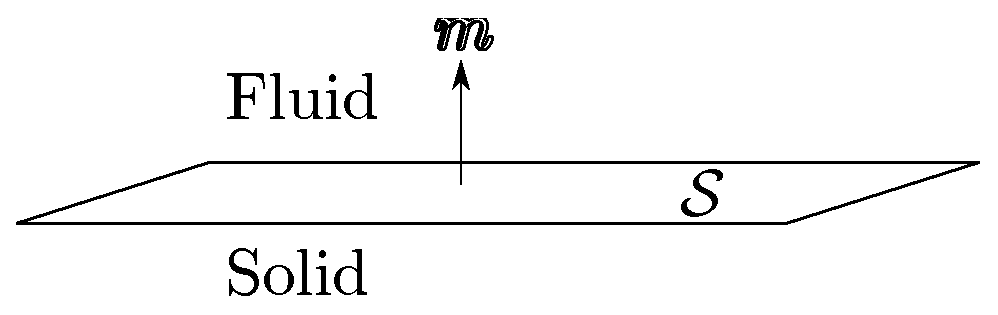
\includegraphics[width=80mm]{fluid_solid.eps}$$
\caption{Fluid-solid boundary $\mathcal{S}$ with normal vector $\boldsymbol{m}$ directed into the fluid phase. \label{fig:fluid-solid_boundary}}
\end{figure}

This is valid for situations when the fluid domain is much larger than the mean free path of molecules within the fluid. When this isn't true, a slip condition can be employed at the boundary \citep{Dussan76}. There also needs to be a dynamic boundary condition applied at the interface. If the solid exerts a force $F_{i}$ onto the fluid, then the condition states

\begin{equation}
\label{equ:dyn_fluid_solid}
\int_{\mathcal{S}} m_{i}(\boldsymbol{x}) T_{ij}(\boldsymbol{x}) \mathrm{d} \mathcal{S} = F_{j} ,
\end{equation}

where $m_{i}(\boldsymbol{x})$ is the normal vector to $\mathcal{S}$ directed into the fluid. Using the non-dimensionalisation scheme presented above this becomes

\begin{equation}
\label{equ:nodim_fluid_solid}
\eta_{\text{c}} U_{\text{c}} L_{\text{c}} \int_{\mathcal{S}} f_{i}(\boldsymbol{x'}) \mathrm{d} \mathcal{S'} = F_{i} ,
\end{equation}

where $f_{i}(\boldsymbol{x'}) =m_{i}(\boldsymbol{x'}) T'_{ij}(\boldsymbol{x'})$ is defined as the dimensionless traction vector on the surface $\mathcal{S}$, .

\subsubsection{Fluid-Fluid Boundary}
\label{subsubsec:BC_fluid-fluid}

For a boundary $\mathcal{I}$ between two fluids labelled 1 and 2 (figure~\ref{fig:fluid-fluid_boundary}), the usual kinematic boundary condition states that the velocity of the two fluids must be continuous across the interface \citep{Kim05}. Defining the velocity of fluid $l$ as $u_{l}$ this can be expressed in dimensionless form as

\begin{equation}
\label{equ:fluid_fluid_kin}
u'_{1,i}(\boldsymbol{x'}) = u'_{2,i}(\boldsymbol{x'}), \quad \text{for } \boldsymbol{x'} \in \mathcal{I} .
\end{equation}

\begin{figure}
$$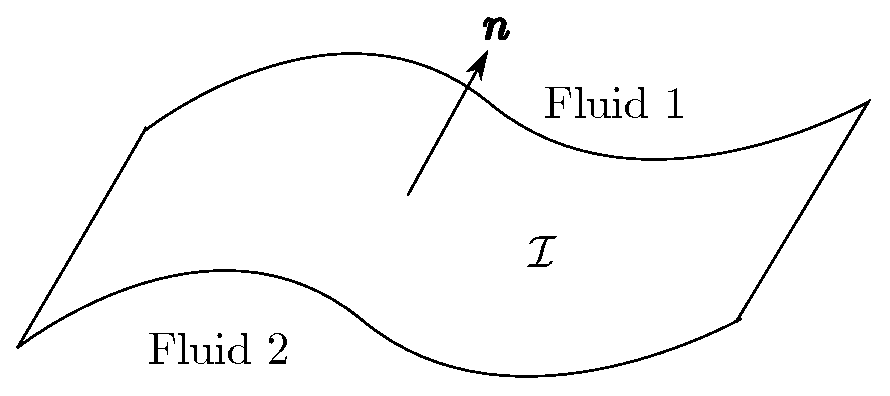
\includegraphics[width=80mm]{fluid_fluid.eps}$$
\caption{Fluid-fluid boundary $\mathcal{I}$ with normal vector $\boldsymbol{n}$. \label{fig:fluid-fluid_boundary}}
\end{figure}

Again, when fluid domains are small compared to the mean free path of molecules a slip condition can be employed \citep{Maxwell1879}. The dynamic boundary condition is an expression of the balance between the stress discontinuity across the interface and the interfacial tension (IFT) $\sigma$ \citep{Batchelor67}. With our definition of the stress tensor this is given as \citep{Manga94}

\begin{align}
\label{equ:fluid_fluid_dyn}
n_{i}(\boldsymbol{x}) [T_{1,ij}(\boldsymbol{x}) - \rho_{1} g_{k} x_{k} \delta_{ij}] - n_{i}(\boldsymbol{x}) [T_{2,ij}(\boldsymbol{x}) - \rho_{2} g_{k} x_{k} \delta_{ij}] = \\ \nonumber
\sigma(\boldsymbol{x}) n_{j}(\boldsymbol{x}) [\partial_{\text{s},i} n_{i}(\boldsymbol{x})] - \partial_{\text{s},j} \sigma (\boldsymbol{x}) , \quad \text{for } \boldsymbol{x} \in \mathcal{I} ,
\end{align}

where $n_{i}$ is the normal vector to the surface $\mathcal{I}$ directed into fluid 1. The operator $\partial_{\text{s},i}$ is defined as the tangential gradient operator within the surface $\mathcal{I}$:

\begin{equation}
\label{equ:surf_grad}
\partial_{\text{s},i} = (\delta_{ij} - \partial_{i} \partial_{j}) \partial_{j} .
\end{equation}

When this takes the normal vector as its argument it can be shown that \citep{Brackbill92}

\begin{equation}
\label{equ:tang_diff_norm}
\partial_{\text{s},i} n_{i} = \partial_{i} n_{i}.
\end{equation}

The presence of spatial gradients in the interfacial tension can lead to so-called Marangoni effects \citep{Thomson1855, Gibbs1878}. However, for our purposes we will assume that the interfacial tension is uniform across the interface $\mathcal{I}$, and so the last term on the right hand side vanishes;

\begin{align}
\label{equ:fluid_fluid_dyn_nograd}
n_{i}(\boldsymbol{x}) [{T}_{1,ij} (\boldsymbol{x}) - \rho_{1} g_{k} x_{k} \delta_{ij}] - n_{i} [T_{2,ij}(\boldsymbol{x}) - \rho_{2} g_{k} x_{k} \delta_{ij}] = \\ \nonumber
\sigma(\boldsymbol{x}) n_{i}(\boldsymbol{x}) \partial_{i} n_{j}(\boldsymbol{x}),  \quad \text{for }\boldsymbol{x} \in \mathcal{I}.
\end{align}

Like the equations of motion, this can be non-dimensionalised using equations~\ref{equ:nodim_l} to~\ref{equ:nodim_T}

\begin{equation}
\label{equ:nodim_fluid_fluid_dyn}
n_{i}(\boldsymbol{x'}) [T'_{1,ij}(\boldsymbol{x'}) - T'_{2,ij}(\boldsymbol{x'})] \Ca + \Bo (\hat{z}_{i} x'_{i}) n_{j}(\boldsymbol{x'}) = n_{j}(\boldsymbol{x'}) \partial'_{i} n_{i}(\boldsymbol{x'}) \quad \text{for }\boldsymbol{x'} \in \mathcal{I}.
\end{equation}

The capillary number $\Ca$ and  Bond number $\Bo$ are dimensionless numbers defined as:

\begin{equation}
\label{equ:cap}
\Ca = \frac{\eta_{\text{c}} U_{\text{c}}}{\sigma},
\end{equation}

and

\begin{equation}
\label{equ:Bond}
\Bo = \frac{(\rho_{2} - \rho_{1}) g L_{\text{c}}^{2}}{\sigma}.
\end{equation}

\subsection{Greens functions}
\label{subsec:BIE_deriv}

In order to derive the integral representation of the Stokes equations, it is necessary to make use of the Greens functions \citep{Riley06} for Stokes flow, $\hat{u}_{i}(\boldsymbol{x'} - \boldsymbol{y'})$ and $\hat{T}_{ij}(\boldsymbol{x'} - \boldsymbol{y'})$, defined such that \citep{Kim05}

\begin{equation}
\label{equ:vel_green_def}
\partial'_{i} \hat{u}_{i}(\boldsymbol{x'} - \boldsymbol{y'}) = 0,
\end{equation}

and

\begin{equation}
\label{equ:stress_green_def}
\partial'_{i} \hat{T}_{ij}(\boldsymbol{x'} - \boldsymbol{y'}) + \mathcal{F}_{j} \delta(\boldsymbol{x'} - \boldsymbol{y'}) = 0 , 
\end{equation}

where $\mathcal{F}_{i}$ is a arbitrary constant vector, $\delta(\boldsymbol{x'} - \boldsymbol{y'})$ is the Dirac delta-function (appendix~\ref{app:delta}) and both $\hat{u}_{i}(\boldsymbol{x'})$ and $\hat{T}_{ij}(\boldsymbol{x'}) \to 0$ as $|\boldsymbol{x'}| \to \infty$. Equations~\ref{equ:vel_green_def} and~\ref{equ:stress_green_def} can be solved following \citet{Ladyzhenskaya63} to show that (see appendix~\ref{app:Greens}) \citep{Kim05}

\begin{equation}
\label{equ:vel_green}
\hat{u}_{j}(\boldsymbol{\xi}) = \frac{ \mathcal{F}_{i} J_{ij}(\boldsymbol{\xi})}{\Lambda} ,
\end{equation}

and 

\begin{equation}
\label{equ:stress_green}
\hat{T}_{ij}(\boldsymbol{\xi}) = K_{ijk}(\boldsymbol{\xi}) \mathcal{F}_{k} ,
\end{equation}

where $\boldsymbol{\xi} = \boldsymbol{x'} - \boldsymbol{y'}$,

\begin{equation}
\label{equ:J_kernal}
J_{ij}(\boldsymbol{\xi}) = \frac{1}{8 \pi \xi} \left( \delta_{ij} + \frac{\xi_{i} \xi_{j}}{\xi^{2}} \right) ,
\end{equation}

and

\begin{equation}
\label{equ:K_kernal}
K_{ijk}(\boldsymbol{\xi}) = \frac{-3 \xi_{i} \xi_{j} \xi_{k}}{4 \pi \xi^{5}}.
\end{equation}

We have defined $\xi = \xi_{i} \xi_{i}$.

\subsection{Integral Representation of Stokes Equations}
\label{subsec:int_rep}

We now substitute the Greens functions and unknown velocity and stress field solutions into the Lorentz Reciprocal Theorem (equation~\ref{equ:LRT} in appendix~\ref{app:Lorentz}) and simplfify using equations~\ref{equ:Stokes} and~\ref{equ:stress_green_def} to find

\begin{equation}
\label{equ:gen_int_rep}
\dashint_{\mathcal{V}} u'_{k}(\boldsymbol{x'}) \delta(\boldsymbol{\xi}) \mathrm{d} \boldsymbol{x'}^{3} = \frac{1}{\Lambda} \dashint_{\mathcal{S}} J_{ik}(\boldsymbol{\xi}) T'_{ij}(\boldsymbol{x'}) n_{j}(\boldsymbol{x'}) \mathrm{d} \boldsymbol{x'}^{2} - \dashint_{\mathcal{S}} u'_{i}(\boldsymbol{x'}) K_{ijk}(\boldsymbol{\xi}) n_{j}(\boldsymbol{x'}) \mathrm{d} \boldsymbol{x'}^{2} .
\end{equation}

Here the integrals are defined in the sense of the Cauchy Principle Value (CPV) to account for the possibility that the kernels $J_{ij}$ and $K_{ijk}$ have singular points in the range of integration. Finally make the transformation $\boldsymbol{x'} \leftrightarrow \boldsymbol{y'}$ and use the symmetry properties of the kernels (equations~\ref{equ:j_sym} and~\ref{equ:k_sym} in appendix~\ref{app:Greens}) and the delta function (equation~\ref{equ:delta_sym} in appendix~\ref{app:delta}) to obtain the general form of the integral representation of the Stokes equations;

\begin{equation}
\label{equ:Stokes_int}
\dashint_{\mathcal{V}} u'_{k}(\boldsymbol{y'}) \delta(\boldsymbol{\xi}) \mathrm{d} \boldsymbol{y'}^{3} = \frac{1}{\Lambda} \dashint_{\mathcal{S}} J_{ik}(\boldsymbol{\xi}) T'_{ij}(\boldsymbol{y'}) n_{j}(\boldsymbol{y'}) \mathrm{d} \boldsymbol{y'}^{2} + \dashint_{\mathcal{S}} u'_{i}(\boldsymbol{y'}) K_{ijk}(\boldsymbol{\xi}) n_{j}(\boldsymbol{y'}) \mathrm{d} \boldsymbol{y'}^{2} .
\end{equation}

Using the definition of the delta function (equation~\ref{equ:dirac} in appendix~\ref{app:delta}) this means

\begin{equation}
\label{equ:Stokes_int_domain}
\frac{1}{\Lambda} \dashint_{\mathcal{S}} J_{ik}(\boldsymbol{\xi}) T'_{ij}(\boldsymbol{y'}) n_{j}(\boldsymbol{y'}) \mathrm{d} \boldsymbol{y'}^{2} + \dashint_{\mathcal{S}} u'_{i}(\boldsymbol{y'}) K_{ijk}(\boldsymbol{\xi}) n_{j}(\boldsymbol{y'}) \mathrm{d} \boldsymbol{y'}^{2} = 
\left\{
    \begin{array}{l l}
      u'_{k}(\boldsymbol{x'}) &\quad \boldsymbol{x'} \in \mathcal{V} \\
      \frac{u'_{k}(\boldsymbol{x'})}{2} &\quad \boldsymbol{x'} \in \mathcal{S} \\
      0 & \quad \text{otherwise}
\end{array}
\right.\ .
\end{equation}

\section{Theoretical Development}
\label{sec:theory}

\subsection{Problem Statement}
\label{subsec:theory}

We are interested in the low Reynolds number, on-axis gravitational settling of a spheroid towards a fluid-fluid interface (figure~\ref{fig:params}). We denote the upper(lower) phase as fluid 1(2). The physical parameters motivate the choice of scaling variables. The characteristic lengthscale is chosen to be the horizontal minor axis $a$, characteristic viscosity that of the upper fluid $\eta_{1}$, and characteristic velocity to be the terminal velocity of a sphere of radius $a$ in the upper fluid\citep{Reynolds1886}

\begin{equation}
\label{equ:char_vel}
U_{\text{c}} = \frac{2 (\rho_{\text{s}} - \rho_{1}) g a^{2}}{9 \eta_{1}} ,
\end{equation}

where $\rho_{1}$ is the density of fluid 1, $\rho_{\text{s}}$ the spheroid density, and $g = 9.81$ m s$^{-1}$ the acceleration due to gravity. Defining $\rho_{2}$ as the density of fluid 2 and $\sigma$ as the IFT, this means the capillary and Bond numbers can be expressed as

\begin{equation}
\label{equ:cap_spec}
\Ca = \frac{(\rho_{\text{s}} - \rho_{1}) g a^{2}}{\sigma},
\end{equation}

and

\begin{equation}
\label{equ:bond_spec}
\Bo = \frac{(\rho_{2} - \rho_{1}) g a^{2}}{\sigma}.
\end{equation}


  \begin{figure}
    $$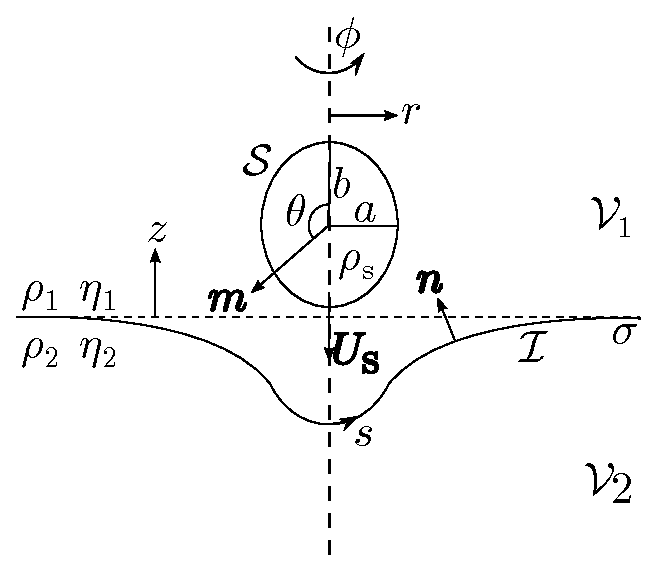
\includegraphics[width=0.8\textwidth]{formulation.eps}$$
    \caption{Diagrammatic representation of the system. A spheroid falls on-axis under gravity, at low Reynolds number, towards an initially horizontal interface between two density stratified, immiscible, semi-infinite fluids. \label{fig:params}}
  \end{figure}


The dimensionless stress tensor for each fluid can be written as

\begin{equation}
\label{equ:nd_stress_def}
T_{\alpha, ij}'(\boldsymbol{x'}) = -P_{\text{d},l}'(\boldsymbol{x'}) \delta_{ij} + \Lambda_{l}[\partial_{i}' u_{l, j}'(\boldsymbol{x'}) - \partial_{j}' u_{l, i}'(\boldsymbol{x'})],
\end{equation}

where $P'_{\text{d},l}$ and $u'_{l,i}$ are the dimensionless dynamic pressure and velcoity fields in fluid $l$ respectively. We use $l$ to denote the fluid and $i,j$ to denote tensoral components. The parameter $\Lambda_{l}$ is defined as

\begin{equation}
\label{equ:Llambda}
\Lambda_{l} = \frac{\eta_{l}}{\eta_{1}} = \left\{
    \begin{array}{l l}
      1, & \quad l = 1 \\
      \frac{\eta_{2}}{\eta_{1}} = \lambda, & \quad l = 2
    \end{array} \right.\ .
\end{equation}

where $\eta_{2}$ is the dynamic viscosity of the lower phase. Note $\lambda$ is the viscosity ratio of the two fluids. Additionally $\mathcal{V}_{1(2)}$ dentotes the volume of fluid 1(2), $\mathcal{I}$ the interface and $\mathcal{S}$ the spheroid surface. $\boldsymbol{m}$ and $\boldsymbol{n}$ are the normal vectors to the spheroid surface and interface respectively and both are directed into fluid 1. We use cylindrical polar coordinates to describe the system with $r$ the radial coordinate with respect to the symmetry axis, $\phi$ the azimuthal coordinate, and $z$ the vertical coordinate with respect to the plane of the initial, undeformed interface. Additionally we make use of the polar angle $\theta$ defined with respect to the centre of the spheroid, and the arc-length $s$ defined as the distance along the interface from the symmetry axis in any azimuthal plane.

It is straightforward to apply the general equations of motion and boundary conditions to the problem. The equations of motion, which must be satsified in both fluid domains, appear as 

\begin{equation}
\label{equ:cont}
\partial_{\text{i}}' u_{l,i}'(\boldsymbol{x'}) = 0,
\end{equation}

and 

\begin{equation}
\label{equ:prob_stokes}
\partial_{\text{i}}' T_{l,ij}'(\boldsymbol{x'}) = 0.
\end{equation}

The first boundary condition that we impose is that the undisturbed fluid is quiescent, so the velocity field is constrained to decay away from the sphere;

\begin{equation}
\label{equ:BC_inf}
u_{l, i}'(\boldsymbol{x'}) \to 0 \text{ as } |\boldsymbol{x'}| \to \infty.
\end{equation}

The kinematic boundary condition on the fluid interface (equation~\ref{equ:fluid_fluid_kin}) can be expressed as  

\begin{equation}
\label{equ:BC_kin_int_nodim}
u_{1,i}'(\boldsymbol{x'}) = u_{2,i}'(\boldsymbol{x'}), \quad \boldsymbol{x'} \in \mathcal{I}.
\end{equation}

The dynamic boundary condition is also imposed at the interface;

\begin{equation}
\label{equ:BC_dyn_int}
n_{i}(\boldsymbol{x'}) [T_{1, ij}'(\boldsymbol{x'}) - T_{2,ij}'(\boldsymbol{x'})] \Ca + \hat{z}_{i} x_{i}' n_{j}(\boldsymbol{x'}) \Bo = n_{j}(\boldsymbol{x'}) \partial_{i}' n_{i}(\boldsymbol{x'}), \quad \text{for } \boldsymbol{x'} \in \mathcal{I}.
\end{equation}

However we can define the modified density ratio (MDR) D as

\begin{equation}
\label{equ:dim_dens_rat}
D = \frac{\Ca}{\Bo} = \frac{\rho_{\text{s}} - \rho_{1}}{\rho_{2} - \rho_{1}}.
\end{equation}

This means equation~\ref{equ:BC_dyn_int} can be re-expressed as

\begin{equation}
\label{equ:d_int}
n_{i}(\boldsymbol{x'}) [T_{1, ij}'(\boldsymbol{x'}) - T_{2, ij}'(\boldsymbol{x'})] D \Bo = n_{j}(\boldsymbol{x'})[\partial_{i}' n_{i}(\boldsymbol{x'}) - \hat{z}_{i} x_{i}' \Bo] , \quad \text{for } \boldsymbol{x'} \in \mathcal{I}.
\end{equation}

The kinematic boundary condition on the spheroid surface is 

\begin{equation}
\label{equ:BC_kin_spere}
u_{1,i}'(\boldsymbol{x'}) = U_{\text{s},i}', \quad \boldsymbol{x'} \in \mathcal{S}.
\end{equation}

where $U_{\text{s},i}$ is the velocity of the spheroid. The final boundary condition is the dynamic boundary condition on the spheroid. The force on the fluid due to the spheroid originates from the balance between gravity and buoyancy;

\begin{equation}
\label{equ:sphere_force}
F_{i} = -\frac{4 \pi a^{2} b (\rho_{\text{s}} - \rho_{1}) g \hat{z}_{i}}{3},
\end{equation}

where b is the vertical minor axis. Substituting this into equation~\ref{equ:nodim_fluid_solid} and using equation~\ref{equ:char_vel} we obtain

\begin{equation}
\label{equ:BC_dyn_sphere}
\int_{\mathcal{S}} f_{i}(\boldsymbol{x'}) \mathrm{d} \mathcal{S}' = -6 \pi \hat{z}_{i}.
\end{equation}

Defining the aspect ratio of the spheroid $R = b / a$, the dimensionless numbers that describe the system are the set $\{\lambda, D, \Bo, R\}$.

\subsection{Integral Representation}
\label{subsec:prob_int_rep}

To recast the problem in an integral representation, we need to apply equation~\ref{equ:Stokes_int_domain} to each fluid separately. The domain of fluid 1 is bound by the spheroid surface and interface, and extends to infinity as $r, z \to \infty$. The boundary condition at infinity (equation~\ref{equ:BC_inf}) ensures that the far-field contribution to the surface integrals in equation~\ref{equ:Stokes_int_domain} vanishes, meaning that just the spheroid surface and interface contribute. Additionally the no-slip boundary condition on the spheroid surface (equation~\ref{equ:BC_kin_spere}), the divergence theorem (appendix~\ref{app:div_theory}) and the definition of the Greens function for pressure (equation~\ref{equ:stress_green_def}) can be used to show that the integral of $u'_{1,i}(\boldsymbol{y'}) K_{ijk}(\boldsymbol{\xi}) m_{j}(\boldsymbol{y'})$ over the spheroid surface vanishes. Hence the boundary integral equation for fluid 1 can be written as 


\begin{align}
\label{equ:bie_fluid1}
\dashint_{\mathcal{S}} J_{ik}(\boldsymbol{\xi}) T'_{1,ij}(\boldsymbol{y'}) m_{j}(\boldsymbol{y'}) \mathrm{d}^{2} \boldsymbol{y'} + \dashint_{\mathcal{I}} J_{ik}(\boldsymbol{\xi}) T'_{1,ij}(\boldsymbol{y'}) n_{j}(\boldsymbol{y'}) \mathrm{d}^{2}\boldsymbol{y'} + \nonumber \\
\dashint_{\mathcal{I}} u'_{1,i}(\boldsymbol{y'}) K_{ijk}(\boldsymbol{\xi}) n_{j}(\boldsymbol{y}) \mathrm{d}^{2}\boldsymbol{y'} = 
\left\{
    \begin{array}{l l}
      \frac{u'_{1,k}(\boldsymbol{x'})}{2} &\quad \boldsymbol{x'} \in \mathcal{I} \\
      u'_{s,k} &\quad \boldsymbol{x'} \in \mathcal{S} 
\end{array}
\right.\ .
\end{align}

For fluid 2, the contribution to the surface integrals at infinity again vanishes leaving just a contribution from the interface. Using the kinemtic boundary condition at the interface (equation~\ref{equ:BC_kin_int_nodim}) the boundary integral equation for fluid 2 can be written as

\begin{equation}
\label{equ:bie_fluid2}
-\dashint_{\mathcal{I}} J_{ik}(\boldsymbol{\xi}) T'_{1,ij}(\boldsymbol{y'}) n_{j}(\boldsymbol{y'}) \mathrm{d}^{2}\boldsymbol{y'} - \lambda \dashint_{\mathcal{I}} u'_{1,i}(\boldsymbol{y'}) K_{ijk}(\boldsymbol{\xi}) n_{j}(\boldsymbol{y}) \mathrm{d}^{2}\boldsymbol{y'} = \frac{\lambda u'_{1,k}(\boldsymbol{x'})}{2} \quad \boldsymbol{x'} \in \mathcal{I} ,
\end{equation}

where the minus sign occurs since the normal vector is directed out of fluid 2. Equations~\ref{equ:bie_fluid1} and~\ref{equ:bie_fluid2} can be added together and combined with equation~\ref{equ:d_int} to obtain

\begin{align}
\label{equ:I1}
\dashint_{\mathcal{S}} J_{ik}(\boldsymbol{\xi}) f_{\text{s},i}(\boldsymbol{y'}) \mathrm{d}^{2} \boldsymbol{y'} + \frac{9}{2 D \text{Bo}} \dashint_{\mathcal{I}} J_{ik}(\boldsymbol{\xi}) n_{i}(\boldsymbol{y'}) [\partial'_{j} n_{j}(\boldsymbol{y'}) - \hat{z}_{j} y'_{j} \text{Bo}] \mathrm{d}^{2} \boldsymbol{y'} + \nonumber \\
(1 - \lambda) \dashint_{\mathcal{I}} u'_{1,i}(\boldsymbol{y'}) K_{ijk}(\boldsymbol{\xi}) n_{j}(\boldsymbol{y'}) \mathrm{d}^{2}\boldsymbol{y'} = 
\left\{
    \begin{array}{l l}
      \frac{(1 + \lambda) u'_{1,k}(\boldsymbol{x'})}{2} &\quad \boldsymbol{x'} \in \mathcal{I} \\
      u'_{s,k} &\quad \boldsymbol{x'} \in \mathcal{S} 
\end{array}
\right.\ .
\end{align}

This together with equation~\ref{equ:BC_dyn_sphere} completely describes the system in an integral representation. 

\subsection{Axisymmetric Simplification}
\label{subsec:axi_sym}

We can exploit the axial symmetry of the system to chose the point $\boldsymbol{x'}$ such that it lies in the plane defined by $\phi = 0$. Hence in Cartesian coordinates $\boldsymbol{x'} = (x_{r}, 0, x_{z})$. This also means we can write $\boldsymbol{y'} = (y_{r} \cos \phi, y_{r} \sin \phi, y_{z})$. On the surface of the spheroid $y_{r} = y_{r}(\theta)$ and $y_{z} = y_{z}(\theta)$, and on the interface $y_{r} = y_{r}(s)$ and $y_{z} = y_{z}(s)$. Additionally $\boldsymbol{f}_{} = [f_{r}(\theta) \cos \phi, f_{r}(\theta) \sin \phi, f_{z}(\theta)]$ and $\boldsymbol{n} = [n_{r}(s) \cos\phi, n_{r}(s) \sin\phi, n_{z}(s)]$. Since the system is axisymmetric, it is useful to extract the azimuthal integration from the surface integrals in equations~\ref{equ:BC_dyn_sphere} and~\ref{equ:I1}. To achieve this, the Cartesian components of each equation are considered separately. For equation~\ref{equ:I1}, it can be shown that both the left and right hand sides of the 2-component equation are identically zero. For equation~\ref{equ:BC_dyn_sphere} this is true for the 1- and 2-components. To show this, $J_{ij}$ and $K_{ijk}$ are first expanded in terms of in terms of the components of $\boldsymbol{x'}$ and $\boldsymbol{y'}$ before the integration over $\phi$ is carried out. This leaves three integral equations which can be expressed as

\begin{align}
\label{equ:cont_ie_1}
R \int_{\theta = 0}^{\pi} B_{\alpha\beta}(\boldsymbol{x'},\theta) \Phi_{\beta}(\theta) \mathrm{d}\theta + \int_{s = 0}^{\infty} \left(A_{\alpha\beta}(\boldsymbol{x'},s) y_{r}(s) - \frac{(1 + \lambda)\delta_{\alpha\beta} \delta(s - s_{0})}{2}\right) \Psi_{\beta}(s) \mathrm{d}s \nonumber \\
= - \int_{s = 0}^{\infty} C_{\alpha}(\boldsymbol{x'},s) y_{r}(s) \mathrm{d}s, \quad \text{for } \boldsymbol{x'} \in \mathcal{I},
\end{align}

\begin{equation}
\label{equ:cont_ie_2}
R \int_{\theta = 0}^{\pi} B_{\alpha\beta}(\boldsymbol{x'},\theta) \Phi_{\beta}(\theta) \mathrm{d}\theta + \int_{s = 0}^{\infty} A_{\alpha\beta}(\boldsymbol{x'},s) \Psi_{\beta}(s) y_{r}(s) \mathrm{d}s - \Theta_{\alpha} = \int_{s = 0}^{\infty} C_{\alpha}(\boldsymbol{x'},s) y_{r}(s) \mathrm{d}s, \quad \text{for } \boldsymbol{x'} \in \mathcal{S}, 
\end{equation}

and 

\begin{equation}
\label{equ:cont_ie_3}
\int_{\theta = 0}^{\pi} \Phi_{2}(\theta) \mathrm{d}\theta = -3, 
\end{equation}

where the quantities $\boldsymbol{A}$, $\boldsymbol{B}$, $\boldsymbol{C}$, $\boldsymbol{\Psi}$, $\boldsymbol{\Phi}$ and $\boldsymbol{\Theta}$ are defined as:

\begin{equation}
\setlength{\arraycolsep}{5pt}
\renewcommand{\arraystretch}{1.3}
\boldsymbol{A} = (1 - \lambda) \bigint_{\phi = 0}^{2 \pi} \left( \begin{matrix}
   n_{r}(K_{111} \cos^{2}\phi + K_{221} \sin^{2}\phi + 2 K_{121} \sin\phi \cos\phi) &  n_{r}(K_{131} \cos\phi + K_{231} \sin\phi)   \\[-15pt]
{}+n_{z}(K_{131} \cos\phi + K_{231} \sin\phi) & {}+n_{z}K_{331} \\[-5pt]
   n_{r}(K_{113} \cos^{2}\phi + K_{223} \sin^{2}\phi + 2 K_{123} \sin\phi \cos\phi) &   n_{r}(K_{133} \cos\phi + K_{233} \sin\phi)  \\[-15pt]
{}+n_{z}(K_{133} \cos\phi + K_{233} \sin\phi) & {}+n_{z}K_{333} \\
\end{matrix} \right) \mathrm{d}\phi ,
\label{equ:mat_A}
\end{equation}


\begin{equation}
\setlength{\arraycolsep}{5pt}
\renewcommand{\arraystretch}{1.3}
\boldsymbol{B} = \bigintss_{\phi = 0}^{2 \pi} \left( \begin{matrix}
J_{11} \cos\phi + J_{21} \sin\phi & J_{31} \\[-5pt]
J_{13} \cos\phi + J_{23} \sin\phi & J_{33} \\
\end{matrix} \right) \mathrm{d}\phi ,
\label{equ:mat_B}
\end{equation}


\begin{equation}
\setlength{\arraycolsep}{5pt}
\renewcommand{\arraystretch}{1.3}
\boldsymbol{C} = \frac{9(\partial'_{j} n_{j} - \text{Bo} y_{z})}{2 D \text{Bo}} \bigintss_{\phi = 0}^{2 \pi} \left( \begin{matrix}
n_{r} (J_{11} \cos\phi + J_{21} \sin\phi) + n_{z} J_{31} \\[-5pt]
n_{r} (J_{13} \cos\phi + J_{23} \sin\phi) + n_{z} J_{23} \\
\end{matrix} \right) \mathrm{d}\phi ,
\label{equ:mat_C}
\end{equation}


\begin{equation}
\setlength{\arraycolsep}{5pt}
\renewcommand{\arraystretch}{1.3}
\boldsymbol{\Psi} = \left( \begin{matrix}
u'_{1,r}(s) \\[-5pt]
u'_{1,z}(s) \\
\end{matrix} \right),
\label{equ:vec_a}
\end{equation}


\begin{equation}
\setlength{\arraycolsep}{5pt}
\renewcommand{\arraystretch}{1.3}
\boldsymbol{\Phi} = \left( \begin{matrix}
f_{\text{s},r}(\theta) \\[-5pt]
f_{\text{s},z}(\theta) \\
\end{matrix} \right) \sin^{2}\theta \left(1 + \frac{\cot^{2}\theta}{R^{2}}\right)^{1/2}  ,
\label{equ:vec_b}
\end{equation}

and 

\begin{equation}
\setlength{\arraycolsep}{5pt}
\renewcommand{\arraystretch}{1.3}
\boldsymbol{\Theta} = \left( \begin{matrix}
0 \\[-5pt]
u'_{\text{s}} \\
\end{matrix} \right) 
\label{equ:vec_d}
\end{equation}

For brevity, the function arguments have been dropped from the kernels and the normal vectors but $n_{i} = n_{i}[\boldsymbol{y'}(s, \phi)]$ and in equation~\ref{equ:mat_A}, $K_{ijk} = K_{ijk}[\boldsymbol{x'} - \boldsymbol{y'}(s, \phi)]$, in equation~\ref{equ:mat_B}, $J_{ij} = J_{ij}[\boldsymbol{x'} - \boldsymbol{y'}(\theta, \phi)]$ and in equation~\ref{equ:mat_C}, $J_{ij} = J_{ij}[\boldsymbol{x'} - \boldsymbol{y'}(s, \phi)]$.

The aziumthal integrals inside the definitions of $\boldsymbol{A}$, $\boldsymbol{B}$ and $\boldsymbol{C}$ can be expressed as sums of complete elliptic integrals of the first and second kind \citep{Lee82, Geller86, Graziani89, Pozrikidis92, Manga94, Roumeliotis00} which can then be evaluated using polynomial expansions \citep{Abramowitz72}. Details of this are given in appendices~\ref{app:ellip} and~\ref{app:mat_A}.

\section{Numerical Method}
\label{sec:num_meth}

Equations~\ref{equ:cont_ie_1} to~\ref{equ:cont_ie_3} are a coupled set of integral equations for the unknowns $\boldsymbol{\Psi}(s)$, $\boldsymbol{\Phi}(\theta)$ and $\boldsymbol{\Theta}$. These solutions can be found numerically by discretising the system, allowing the integral equations to be expressed as a linear system of algerbraic equations which are then solved using LU decomposition and Gaussian elimination \citep{Riley06, Press07}. Once the interfacial and sphere velocities are solved for, the system is iterated forward in time, and the process is repeated. 

\subsection{Discretisation and Linear System}
\label{subsec:discrete}

To discretise the set of equations, the interface and sphere surface are divided into intervals. The interface is divided into $N$ axisymmetric rings, where the $i^{\text{th}}$ ring is centred at arc-length $s_{i}$ and is of thinkness $\Delta_{s,i}$.  The interface is truncated at the arc-length $s_{N}$. The sphere surface is discretised in $M$ axisymmetric rings, where the $i^{\text{th}}$ ring is centred at polar coordinate $\theta_{i}$ and has a thickness $\Delta_{\theta,i}$. A schematic of the discretisation scheme is depicted in figure~\ref{fig:discrete}. 

  \begin{figure}
    $$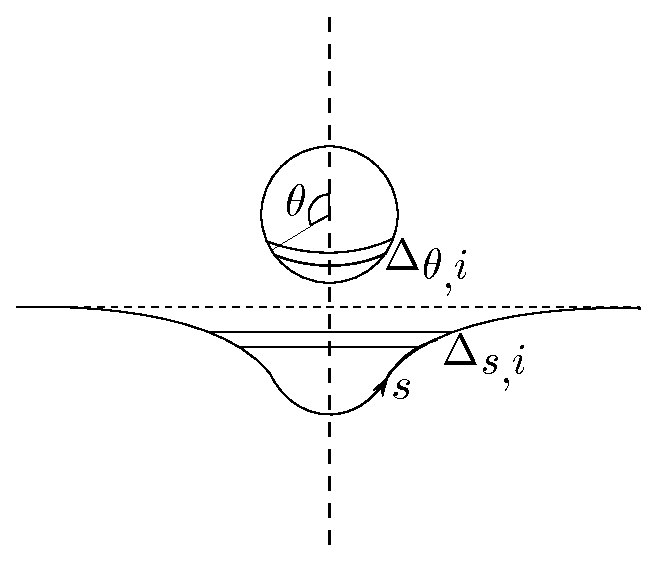
\includegraphics[width=0.8\textwidth]{discrete.eps}$$
    \caption{Diagrammatic representation of the discretisation of the system. Both interface and spheroid surface are divided into axisymmetric rings centred on the symmetry axis. \label{fig:discrete}}
  \end{figure}

We now choose $\boldsymbol{x'} = \boldsymbol{x}_{i}$ where $\boldsymbol{x}_{i} = \boldsymbol{x}_{i}(\theta_{i})$ on $\mathcal{S}$ and $\boldsymbol{x}_{i} = \boldsymbol{x}_{i}(s_{i})$ on $\mathcal{I}$. That is, the point $\boldsymbol{x'}$ is chosen to be the midpoint of one of the intervals. Then, we can express the integrals as discrete sums over each element. We then make the approximation that the unknowns $\boldsymbol{\Psi}(s)$ and $\boldsymbol{\Phi}(\theta)$ are constant over the width of an interval and for interval $i$, $\boldsymbol{\Psi}(s) = \boldsymbol{\Psi}(s_{i})$ and $\boldsymbol{\Phi}(\theta) = \boldsymbol{\Phi}(\theta_{i})$. This allows us to obtain the discrete form of the integral equations:

\begin{align}
\label{equ:dis_ie_1}
R \sum_{i = 1}^{M} \Phi_{\beta}(\theta_{i}) \int_{\Delta_{\theta,i}} B_{\alpha\beta}(s_{j},\theta) \mathrm{d}\theta + \sum_{i=1}^{N} \Psi_{\beta}(s_{i}) \int_{\Delta_{s,i}} \left(A_{\alpha\beta}(s_{j},s) y_{r}(s) - \frac{(1 + \lambda) \delta_{\alpha\beta} \delta(s - s_{j})}{2}\right) \mathrm{d}s \nonumber \\
= - \sum_{i = 1}^{N} \int_{\Delta_{s,i}} C_{\alpha}(s_{j},s) y_{r}(s) \mathrm{d}s,
\end{align}

\begin{equation}
\label{equ:dis_ie_2}
R \sum_{i = 1}^{M} \Phi_{\beta}(\theta_{i}) \int_{\Delta_{\theta,i}} B_{\alpha\beta}(\theta_{j},\theta) \mathrm{d}\theta + \sum_{i=1}^{N} \Psi_{\beta}(s_{i}) \int_{\Delta_{s,i}} A_{\alpha\beta}(\theta_{j},s) y_{r}(s) \mathrm{d}s - \Theta_{\alpha} = - \sum_{i = 1}^{N} \int_{\Delta_{s,i}} C_{\alpha}(\theta_{j},s) y_{r}(s) \mathrm{d}s,
\end{equation}

and 

\begin{equation}
\label{equ:dis_ie_3}
\sum_{i = 1}^{M} \Phi_{2}(\theta_{i}) \int_{\Delta_{\theta,i}} \mathrm{d}\theta = -3.
\end{equation}

This is seemingly a set of $2(N + M) + 1$ linear equations for $2(N + M) + 1$ unknowns; $\Phi_{\alpha}(\theta_{i})$, $\Psi_{\alpha}(s_{j})$ and $\Theta_{1}$ (recall that $\Theta_{2} = 0$) where $\alpha = 1,2$, $i = 1,2,...,M$ and $j = 1,2,...,N$. However we can use physical arguments to simplify the system further. First by symmetry, the radial interfacial velocity must vanish on the symmetry axis i.e. $\Psi_{1}(s_{1}) = 0$. Additionally, the on-axis radial tractions on the sphere must also vanish meaning $\Phi_{1}(\theta_{1}) = \Phi_{1}(\theta_{M}) = 0$. Indeed, it can be shown that the coefficients of these terms vanish by using the expressions for $A_{\alpha\beta}$, $B_{\alpha\beta}$ and $C_{\alpha}$, given in appendix~\ref{subapp:spec_case}. Hence the equations where these terms appear are redundant and can be removed from the linear system. This leaves us with a system of $2(N + M - 1)$ linear equations for $2(N + M - 1)$ unknowns.

\subsection{Evaluation of the coefficients}
\label{subsec:eval_coeff}

These equations can be recast as a matrix equation $L_{\mu\nu} X_{\mu} = Y_{\nu}$ where the unknown quantities are the elements $X_{\mu}$. The elements $L_{\mu\nu}$ and $Y_{\nu}$ are the coefficients of the system and contain integrals that need to be evaluated numerically. If $\boldsymbol{x'}_{j}$ is not within the range of integration, then this is done using 4-point Gaussian-Legendre quadrature \citep{Riley06}. However if $\boldsymbol{x'}_{j}$ is in the integration range, then the integrand is singular at the point $\boldsymbol{y'} = \boldsymbol{x'}_{j}$ and care needs to be taken when evaluating the integral. First, the order of the singularity needs to be determined. To do this, write $\boldsymbol{y'} = \boldsymbol{x'}_{j} + \epsilon \boldsymbol{t}$, where $\epsilon = \theta - \theta_{j}$ on the sphere, and $\epsilon = s - s_{j}$ on the interface, and $\boldsymbol{t}$ is the tangent to the curve. The integrands are then expanded in terms of $\epsilon$. The order of the singularity if the order of the first order singular term in $\epsilon$. Table~\ref{tab:sing} shows the order of the singularity of each component of $\boldsymbol{A}$, $\boldsymbol{B}$ and $\boldsymbol{C}$.

\begin{table}
\centering
\caption{The order of the singularity of the components of $\boldsymbol{A}$, $\boldsymbol{B}$ and $\boldsymbol{C}$. \label{tab:sing}}
\begin{tabular}{|c|c||c|c||c|c|}
  \hline
  $A_{11}$ & $1 / \epsilon$ & $B_{11}$ & $\ln|\epsilon|$ & $C_{1}$  & $\ln|\epsilon|$\\
  $A_{12}$ & 0 & $B_{12}$ & 0 & $C_{2}$  & $\ln|\epsilon|$\\
  $A_{21}$ & 0 & $B_{21}$ & 0  &   & \\
  $A_{22}$ & 0 & $B_{22}$ & $\ln|\epsilon|$ &   & \\
  \hline
\end{tabular} 
\end{table}

We then re-write the integrand as the sum of a regular and singular part. Denoting the integrand by $I(\zeta, \zeta_{i})$ (where $\zeta$ represents $\theta$ or $s$ depending on whether the integration is over the sphere or the interface) this can be written as $I(\zeta, \zeta_{i}) = I_{r}(\zeta, \zeta_{i}) + I_{s}(\zeta, \zeta_{i})$ where $I_{r}$ is the regular part and $I_{s}$ is the singular part. The singular part can then be written as

\begin{equation}
\label{equ:sing_meth}
I(\zeta, \zeta_{i})_{s} = [I_{s}(\zeta, \zeta_{i}) -L(\zeta, \zeta_{i})] + L(\zeta, \zeta_{i}),
\end{equation}

where $L$ is the leading order contribution to $I_{s}$. The terms in square parenthesese now form a regular function which can be integrated numerically. For the case that the integral is $1/\epsilon$ singular, the final term can be expressed as

\begin{equation}
\label{equ:recip_sing}
L(\zeta, \zeta_{i}) = \frac{g(\zeta, \zeta_{i})}{\epsilon} = \frac{g(\zeta, \zeta_{i}) - g(\zeta_{i}, \zeta_{i})}{\epsilon} + \frac{g(\zeta_{i}, \zeta_{i})}{\epsilon}.
\end{equation}

Similarly, if the integral if $\ln|\epsilon|$ singular

\begin{equation}
\label{equ:ln_sing}
L(\zeta, \zeta_{i}) = g(\zeta, \zeta_{i}) \ln|\epsilon| = [g(\zeta, \zeta_{i}) - g(\zeta_{i}, \zeta_{i})]\ln|\epsilon| + g(\zeta_{i}, \zeta_{i})\ln|\epsilon|
\end{equation}

In both these cases, the first term on the right hand side is regular and the last term is singular but can be integrated analytically. This means that the irregular integrand can be expressed as the sum of a regular function, that can be integrated numerically, and an irregular function, that can be integrated analytically. 
 
To calculate integrals over the interface, it is necessary to evaluate the components of the normal vector and its divergence at discrete points along the interface. To do this, cubic splines are fitted to the collocation points describing the interface (WAITING FOR DE BOER BOOK TO REF THIS) using routines given in \citet{Press07} so that the interface is described parametrically with $r = r(s)$ and $z = z(s)$. Remembering that for a surface $H(r,z) = z - f(r)$, the components of the normal vector are given by $n_{i} = \partial_{i} H / (\partial_{j}H \partial_{j}H)$ \citep{Riley06}, the following expressions can be obtained

\begin{equation}
\label{equ:norm_rad}
n_{r}(s) = \frac{-\dot{z}}{(\dot{r} + \dot{z})^{1/2}},
\end{equation}

\begin{equation}
\label{equ:norm_vert}
n_{z}(s) = \frac{\dot{r}}{(\dot{r} + \dot{z})^{1/2}},
\end{equation}

and 

\begin{equation}
\label{equ:div_norm}
\partial'_{i} n_{i} = \frac{\dot{z}}{r (\dot{r} + \dot{z})^{1/2}} + \frac{\dot{r} \ddot{z} - \ddot{r} \dot{z}}{(\dot{r} + \dot{z})^{3/2}}.
\end{equation}

These expressions are given in given in \citep{Manga94} except for a minus sign error in the components of the normal. The derivatives of the splines are calculated numerically using routines modified from \citet{Press07}. Once all of the elements $L_{\mu\nu}$ and $Y_{\nu}$ have been calculated the system of equations is solved by Lower-Upper (LU) decomposition and Gaussian elimination \citep{Riley06, Press07} using routines from the GNU Scientific Library (GSL) \citep{Galassi09}.

\subsection{Temporal Iteration}
\label{subsec:time}

The system is iterated forward in time using an explicit first order Euler method \citep{Manga94} with timestep $\Delta t$. This means the position of the sphere $z_{s}$ at time $t + \Delta t$ is found using

\begin{equation}
\label{equ:sphere_it}
z_{s}(t' + \Delta t') = U'_{s}(t) \Delta t',
\end{equation}

and the position of the collocation points on the interface moves according to

\begin{equation}
\label{equ:int_it}
x_{r}(s_{i}, t' + \Delta t') = u_{r}(s_{i},t') \Delta t',
\end{equation}

and

\begin{equation}
\label{equ:int_it}
x_{z}(s_{i}, t' + \Delta t') = u_{z}(s_{i},t') \Delta t'.
\end{equation}

There are both numerical and physical constraints on the value of the timestep. Numerically, it is limited by the Courant-Friedrich-Lewy (CFL) criterion {Courant28}. Physically, it is neccessary to ensure that it is smaller than the timescale over which different processes can occur. Owing to the multi-component nature of this problem, there are four timescales instrinsic to the problem: the Stokes timescale in the upper fluid $\tau_{\text{s},1} = 9 \eta_{1} / [2 (\rho_{\text{s}} - \rho_{1}) g a]$, the Stokes timescale in the lower fluid $\tau_{\text{s},2} = 9 \eta_{2} / [2 (\rho_{\text{s}} - \rho_{2}) g a]$, the capilary time for the upper fluid $\tau_{\text{c},1} = \eta_{1} a / \sigma$ and the capilary time for the lower fluid $\tau_{\text{c},2} = \eta_{2} a / \sigma$. It is required that the timestep is smaller than all of these so that the physics occuring on each timescale can be resolved. Non-dimensionalising each of these timescales we find that in dimensionless form they exist as $\tau'_{\text{s},1} = 1$, $\tau'_{\text{s},2} = \lambda D / (D - 1)$, $\tau'_{\text{c},1} = 2 D \Bo / 9$, $\tau'_{\text{c},2} = 2 D \Bo \lambda / 9$. Hence, for each simulation, the shortest physical timescale is identified and the timestep is constrained to be smaller than this throughout the simulation. The timestep is allowed to change during the simulation such that it is as large as can be allowed by both the CFL and numerical criteria.


Due to gradients in the velocity tangential to the fluid interface, the distribution of collocation points is altered during this time stepping process, so the collocation points are redistributed between each time step. Following the redistribution, the linear system is reconstructed for the new geometry and solved using the same procedure. The process continues in this fashion until the separtation between the sphere and the interface, or two different parts of the interface equals the local separation between collocation points, as the discretisation no longer provides an accurate approximation to the continuous system


\section{Model Testing}
\label{sec:test}

\subsection{Uniform and Infinite Fluid}
\label{subsec:no_interf}

To test the model, we can remove the interface and fluid 2, leaving us with the problem of the steady gravitational settling of a spheroid through fluid 1, which is uniform and infinite in extent. The terminal velocity of a spheroid settling on axis can be solved for analytically \citep{Happel73} and in our dimensionless scheme is given by

\begin{equation}
\label{equ:term_vel}
U'_{t} = \frac{1}{K},
\end{equation}

where

\begin{equation}
\label{equ:Stokes_corr}
K = \begin{cases}
    \frac{4}{3 (\mu^{2} + 1)^{1/2} [\mu - (\mu^{2} - 1) \cot^{-1} \mu]}       & \quad \text{for } R < 1\\
    \frac{4}{3 (\mu^{2} - 1)^{1/2} [(\mu^{2} + 1) \coth^{-1}\mu - \mu]}  & \quad \text{for } R > 1\\
    1 & \quad \text{for } R = 1, \\
  \end{cases}
\end{equation}

and 

\begin{equation}
\label{equ:Stokes_const}
\mu = \frac{R}{|R^{2} - 1|^{1/2}}.
\end{equation}

For the case that $\lambda = 1$, and a flat interface, the integrals over the interface in equations~\ref{equ:dis_ie_1} to~\ref{equ:dis_ie_3} vanish and the system reduces to that of the case of a spheroid settling in an infinite and uniform fluid. Figure~\ref{fig:Happel_test} shows the analytical result for the terminal velocity from \citet{Happel73} compared with that calculated by our model. It can be seen that agreement is excellent for aspect ratios in the range 0.1-10.

  \begin{figure}
    % GNUPLOT: LaTeX picture with Postscript
\begingroup
  \makeatletter
  \providecommand\color[2][]{%
    \GenericError{(gnuplot) \space\space\space\@spaces}{%
      Package color not loaded in conjunction with
      terminal option `colourtext'%
    }{See the gnuplot documentation for explanation.%
    }{Either use 'blacktext' in gnuplot or load the package
      color.sty in LaTeX.}%
    \renewcommand\color[2][]{}%
  }%
  \providecommand\includegraphics[2][]{%
    \GenericError{(gnuplot) \space\space\space\@spaces}{%
      Package graphicx or graphics not loaded%
    }{See the gnuplot documentation for explanation.%
    }{The gnuplot epslatex terminal needs graphicx.sty or graphics.sty.}%
    \renewcommand\includegraphics[2][]{}%
  }%
  \providecommand\rotatebox[2]{#2}%
  \@ifundefined{ifGPcolor}{%
    \newif\ifGPcolor
    \GPcolorfalse
  }{}%
  \@ifundefined{ifGPblacktext}{%
    \newif\ifGPblacktext
    \GPblacktexttrue
  }{}%
  % define a \g@addto@macro without @ in the name:
  \let\gplgaddtomacro\g@addto@macro
  % define empty templates for all commands taking text:
  \gdef\gplbacktext{}%
  \gdef\gplfronttext{}%
  \makeatother
  \ifGPblacktext
    % no textcolor at all
    \def\colorrgb#1{}%
    \def\colorgray#1{}%
  \else
    % gray or color?
    \ifGPcolor
      \def\colorrgb#1{\color[rgb]{#1}}%
      \def\colorgray#1{\color[gray]{#1}}%
      \expandafter\def\csname LTw\endcsname{\color{white}}%
      \expandafter\def\csname LTb\endcsname{\color{black}}%
      \expandafter\def\csname LTa\endcsname{\color{black}}%
      \expandafter\def\csname LT0\endcsname{\color[rgb]{1,0,0}}%
      \expandafter\def\csname LT1\endcsname{\color[rgb]{0,1,0}}%
      \expandafter\def\csname LT2\endcsname{\color[rgb]{0,0,1}}%
      \expandafter\def\csname LT3\endcsname{\color[rgb]{1,0,1}}%
      \expandafter\def\csname LT4\endcsname{\color[rgb]{0,1,1}}%
      \expandafter\def\csname LT5\endcsname{\color[rgb]{1,1,0}}%
      \expandafter\def\csname LT6\endcsname{\color[rgb]{0,0,0}}%
      \expandafter\def\csname LT7\endcsname{\color[rgb]{1,0.3,0}}%
      \expandafter\def\csname LT8\endcsname{\color[rgb]{0.5,0.5,0.5}}%
    \else
      % gray
      \def\colorrgb#1{\color{black}}%
      \def\colorgray#1{\color[gray]{#1}}%
      \expandafter\def\csname LTw\endcsname{\color{white}}%
      \expandafter\def\csname LTb\endcsname{\color{black}}%
      \expandafter\def\csname LTa\endcsname{\color{black}}%
      \expandafter\def\csname LT0\endcsname{\color{black}}%
      \expandafter\def\csname LT1\endcsname{\color{black}}%
      \expandafter\def\csname LT2\endcsname{\color{black}}%
      \expandafter\def\csname LT3\endcsname{\color{black}}%
      \expandafter\def\csname LT4\endcsname{\color{black}}%
      \expandafter\def\csname LT5\endcsname{\color{black}}%
      \expandafter\def\csname LT6\endcsname{\color{black}}%
      \expandafter\def\csname LT7\endcsname{\color{black}}%
      \expandafter\def\csname LT8\endcsname{\color{black}}%
    \fi
  \fi
    \setlength{\unitlength}{0.0500bp}%
    \ifx\gptboxheight\undefined%
      \newlength{\gptboxheight}%
      \newlength{\gptboxwidth}%
      \newsavebox{\gptboxtext}%
    \fi%
    \setlength{\fboxrule}{0.5pt}%
    \setlength{\fboxsep}{1pt}%
\begin{picture}(7200.00,5040.00)%
    \gplgaddtomacro\gplbacktext{%
      \csname LTb\endcsname%
      \put(946,704){\makebox(0,0)[r]{\strut{}$-4$}}%
      \put(946,1213){\makebox(0,0)[r]{\strut{}$-3.5$}}%
      \put(946,1722){\makebox(0,0)[r]{\strut{}$-3$}}%
      \put(946,2231){\makebox(0,0)[r]{\strut{}$-2.5$}}%
      \put(946,2740){\makebox(0,0)[r]{\strut{}$-2$}}%
      \put(946,3248){\makebox(0,0)[r]{\strut{}$-1.5$}}%
      \put(946,3757){\makebox(0,0)[r]{\strut{}$-1$}}%
      \put(946,4266){\makebox(0,0)[r]{\strut{}$-0.5$}}%
      \put(946,4775){\makebox(0,0)[r]{\strut{}$0$}}%
      \put(1078,484){\makebox(0,0){\strut{}$0.1$}}%
      \put(3941,484){\makebox(0,0){\strut{}$1$}}%
      \put(6803,484){\makebox(0,0){\strut{}$10$}}%
    }%
    \gplgaddtomacro\gplfronttext{%
      \csname LTb\endcsname%
      \put(176,2739){\rotatebox{-270}{\makebox(0,0){\strut{}$U_{\text{t}}$}}}%
      \put(3940,154){\makebox(0,0){\strut{}$R$}}%
      \csname LTb\endcsname%
      \put(5816,4602){\makebox(0,0)[r]{\strut{}Analytical}}%
      \csname LTb\endcsname%
      \put(5816,4382){\makebox(0,0)[r]{\strut{}Model Output}}%
    }%
    \gplbacktext
    \put(0,0){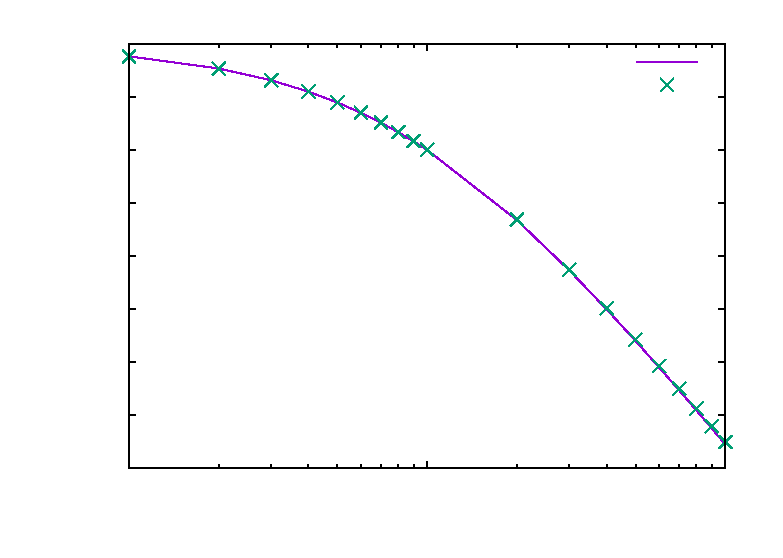
\includegraphics{Happel}}%
    \gplfronttext
  \end{picture}%
\endgroup

    \caption{Curve shows analytical solution for dimensionless terminal velocity vs. aspect ratio (equation~\ref{equ:Stokes_corr}). Points show calculated values from model. There is excellent agreement for oblate spheroids but the error increases with aspect ratio. \label{fig:Happel_test}}
  \end{figure}

We tested the senstivity of the results to the number of intervals on the sphere. Figure~\ref{fig:int_vel_test} shows the fractional error on the calculated terminal velocity as a function of the number of intervals used to discretise the sphere $M$, for both a prolate and oblate spheroid, and a sphere. For $M \geq 100$, the fractional error is less than 0.003. It is also clear here that the error increases with $R$. 

  \begin{figure}
    % GNUPLOT: LaTeX picture with Postscript
\begingroup
  \makeatletter
  \providecommand\color[2][]{%
    \GenericError{(gnuplot) \space\space\space\@spaces}{%
      Package color not loaded in conjunction with
      terminal option `colourtext'%
    }{See the gnuplot documentation for explanation.%
    }{Either use 'blacktext' in gnuplot or load the package
      color.sty in LaTeX.}%
    \renewcommand\color[2][]{}%
  }%
  \providecommand\includegraphics[2][]{%
    \GenericError{(gnuplot) \space\space\space\@spaces}{%
      Package graphicx or graphics not loaded%
    }{See the gnuplot documentation for explanation.%
    }{The gnuplot epslatex terminal needs graphicx.sty or graphics.sty.}%
    \renewcommand\includegraphics[2][]{}%
  }%
  \providecommand\rotatebox[2]{#2}%
  \@ifundefined{ifGPcolor}{%
    \newif\ifGPcolor
    \GPcolorfalse
  }{}%
  \@ifundefined{ifGPblacktext}{%
    \newif\ifGPblacktext
    \GPblacktexttrue
  }{}%
  % define a \g@addto@macro without @ in the name:
  \let\gplgaddtomacro\g@addto@macro
  % define empty templates for all commands taking text:
  \gdef\gplbacktext{}%
  \gdef\gplfronttext{}%
  \makeatother
  \ifGPblacktext
    % no textcolor at all
    \def\colorrgb#1{}%
    \def\colorgray#1{}%
  \else
    % gray or color?
    \ifGPcolor
      \def\colorrgb#1{\color[rgb]{#1}}%
      \def\colorgray#1{\color[gray]{#1}}%
      \expandafter\def\csname LTw\endcsname{\color{white}}%
      \expandafter\def\csname LTb\endcsname{\color{black}}%
      \expandafter\def\csname LTa\endcsname{\color{black}}%
      \expandafter\def\csname LT0\endcsname{\color[rgb]{1,0,0}}%
      \expandafter\def\csname LT1\endcsname{\color[rgb]{0,1,0}}%
      \expandafter\def\csname LT2\endcsname{\color[rgb]{0,0,1}}%
      \expandafter\def\csname LT3\endcsname{\color[rgb]{1,0,1}}%
      \expandafter\def\csname LT4\endcsname{\color[rgb]{0,1,1}}%
      \expandafter\def\csname LT5\endcsname{\color[rgb]{1,1,0}}%
      \expandafter\def\csname LT6\endcsname{\color[rgb]{0,0,0}}%
      \expandafter\def\csname LT7\endcsname{\color[rgb]{1,0.3,0}}%
      \expandafter\def\csname LT8\endcsname{\color[rgb]{0.5,0.5,0.5}}%
    \else
      % gray
      \def\colorrgb#1{\color{black}}%
      \def\colorgray#1{\color[gray]{#1}}%
      \expandafter\def\csname LTw\endcsname{\color{white}}%
      \expandafter\def\csname LTb\endcsname{\color{black}}%
      \expandafter\def\csname LTa\endcsname{\color{black}}%
      \expandafter\def\csname LT0\endcsname{\color{black}}%
      \expandafter\def\csname LT1\endcsname{\color{black}}%
      \expandafter\def\csname LT2\endcsname{\color{black}}%
      \expandafter\def\csname LT3\endcsname{\color{black}}%
      \expandafter\def\csname LT4\endcsname{\color{black}}%
      \expandafter\def\csname LT5\endcsname{\color{black}}%
      \expandafter\def\csname LT6\endcsname{\color{black}}%
      \expandafter\def\csname LT7\endcsname{\color{black}}%
      \expandafter\def\csname LT8\endcsname{\color{black}}%
    \fi
  \fi
    \setlength{\unitlength}{0.0500bp}%
    \ifx\gptboxheight\undefined%
      \newlength{\gptboxheight}%
      \newlength{\gptboxwidth}%
      \newsavebox{\gptboxtext}%
    \fi%
    \setlength{\fboxrule}{0.5pt}%
    \setlength{\fboxsep}{1pt}%
\begin{picture}(7200.00,5040.00)%
    \gplgaddtomacro\gplbacktext{%
      \csname LTb\endcsname%
      \put(1078,704){\makebox(0,0)[r]{\strut{}$0$}}%
      \put(1078,1383){\makebox(0,0)[r]{\strut{}$0.001$}}%
      \put(1078,2061){\makebox(0,0)[r]{\strut{}$0.002$}}%
      \put(1078,2740){\makebox(0,0)[r]{\strut{}$0.003$}}%
      \put(1078,3418){\makebox(0,0)[r]{\strut{}$0.004$}}%
      \put(1078,4097){\makebox(0,0)[r]{\strut{}$0.005$}}%
      \put(1078,4775){\makebox(0,0)[r]{\strut{}$0.006$}}%
      \put(1210,484){\makebox(0,0){\strut{}$50$}}%
      \put(2009,484){\makebox(0,0){\strut{}$100$}}%
      \put(2808,484){\makebox(0,0){\strut{}$150$}}%
      \put(3607,484){\makebox(0,0){\strut{}$200$}}%
      \put(4406,484){\makebox(0,0){\strut{}$250$}}%
      \put(5205,484){\makebox(0,0){\strut{}$300$}}%
      \put(6004,484){\makebox(0,0){\strut{}$350$}}%
      \put(6803,484){\makebox(0,0){\strut{}$400$}}%
    }%
    \gplgaddtomacro\gplfronttext{%
      \csname LTb\endcsname%
      \put(176,2739){\rotatebox{-270}{\makebox(0,0){\strut{}$\Delta U_{\text{t}} / U_{\text{t}}$}}}%
      \put(4006,154){\makebox(0,0){\strut{}$M$}}%
      \csname LTb\endcsname%
      \put(5816,4602){\makebox(0,0)[r]{\strut{}R = 0.5}}%
      \csname LTb\endcsname%
      \put(5816,4382){\makebox(0,0)[r]{\strut{}R = 1}}%
      \csname LTb\endcsname%
      \put(5816,4162){\makebox(0,0)[r]{\strut{}R = 2}}%
    }%
    \gplbacktext
    \put(0,0){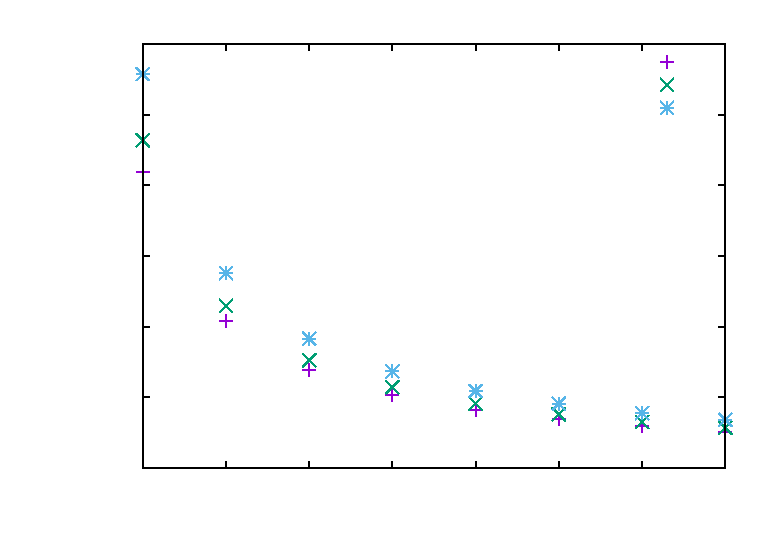
\includegraphics{../../Programming/sinking_bim_write_up/trunk/int_test}}%
    \gplfronttext
  \end{picture}%
\endgroup

    \caption{Plot showing the fractional error on the calculated terminal velocity of a spheroid in an infinite and uniform fluid as a function of the number of intervals used to discretise the particle surface. Results are shown for $R = 0.5$, $1$ and $2$. When 100 intervals are used, the fractional error is less than 0.003 and this decreases as the number of intervals increases. It can also be seen that as $R$ increases so does the error. \label{fig:int_vel_test}}
  \end{figure}

\subsection{Initial Height of Sphere}
\label{subsec:init_pos}

The interface will deform as the particle approaches and so we require the initial position of the particle to be far enough above the interface that the results are insensitive to the initial position. We tested the model for parameter values $R = 1$, $D = 10 $, $\Bo = 1000$ and both $\lambda = 0.1$ and $\lambda = 10$. Figure~\ref{fig:height_test_pos} shows the position of the sphere against time for the different viscosity ratios. The time $t = 0$ is defined as the moment when $z_{\text{s}} = 0$. It is seen that the position curves converge for an initial position greater than or equal to 5 sphere radii above the interface. Figure~\ref{fig:height_vol_test} shows that the same is true when considering the volume of upper phase fluid entrained below the plane $z = 0$.

    \begin{figure}
      \centering
      \begin{subfigure}[b]{0.5\textwidth}
          $$\includegraphics[width=0.6\textwidth, angle=270]{lambda=0_1_height.eps}$$
        \caption{}
        \label{fig:height_test_pos_tail}
      \end{subfigure}%
      ~
      \begin{subfigure}[b]{0.5\textwidth}
        $$\includegraphics[width=0.6\textwidth, angle=270]{lambda=10_height.eps}$$
        \caption{}
        \label{fig:height_test_pos_film}
      \end{subfigure}
      \caption{Plot of the vertical position of a sphere versus time for different initial sphere positions for $D = 10$ and $\Bo = 1000$. a) $\lambda = 0.1$ - For initial positions greater or equal than 5 radii above the interface, the position curves quickly converge. b) $\lambda = 10$ - For initial positions greater or equal than 5 radii above the interface, the position curves are indistingusihable. For an initial position of 3, the curve quickly converges to the others.}\label{fig:height_test_pos}
    \end{figure}

  \begin{figure}
    $$\includegraphics[width=0.4\textwidth, angle=270]{height_vol_test.eps}$$
    \caption{Curves showing the volume of upper phase fluid entrained below the plane $z = 0$ as a function of time, for different initial sphere positions and $D = 10$, $\Bo = 1000$ and $\lambda = 0.1$. It is seen that the curves converge for an initial position greater than or equal to 5 sphere radii above the interface. \label{fig:height_vol_test}}
  \end{figure}

\subsection{Truncation Length}
\label{subsec:trunc_length}

The model is also tested for its sentitivity with respect to the radial coordinate $r = r_{N}$ at which the interface is truncated. Figure~\ref{fig:trunc_test_pos} shows the position of the sphere as a function of time for different $r_{N}$. It is seen that for $r_{N} \geq 10$ there is no change to the results. Figure~\ref{fig:trunc_vol_test} shows the dependence of the entrained volume as a function of time on the truncation radius. For $r_{N} \geq 20$ the curves are identical from the start of the simulation, and for $r_{N} = 10$ the curve converges to the others during the run.


    \begin{figure}
      \centering
      \begin{subfigure}[b]{0.5\textwidth}
          $$\includegraphics[width=0.6\textwidth, angle=270]{lambda=0_1_trunc.eps}$$
        \caption{}
        \label{fig:trunc_test_pos_tail}
      \end{subfigure}%
      ~
      \begin{subfigure}[b]{0.5\textwidth}
        $$\includegraphics[width=0.6\textwidth, angle=270]{lambda=10_trunc.eps}$$
        \caption{}
        \label{fig:trunc_test_pos_film}
      \end{subfigure}
      \caption{Plot of the vertical position of a sphere versus time for different truncation radii for $D = 10$, $\Bo = 1000$ and both $\lambda = 0.1$ (a) and $\lambda = 10$ (b). The curves are identical for all truncation radii greater than or equal to 10.}\label{fig:trunc_test_pos}
    \end{figure}

  \begin{figure}
    $$\includegraphics[width=0.4\textwidth, angle=270]{trunc_vol_test.eps}$$
    \caption{Curves showing the volume of upper phase fluid entrained below the plane $z = 0$ as a function of time, for different truncation radii and $D = 10$, $\Bo = 1000$ and $\lambda = 0.1$. It is seen that the curves for $r_{N} \geq 20$ are identical from the start of the simulation, although the curve for $r_{N} = 10$ converges to the other curves during the run. \label{fig:trunc_vol_test}}
  \end{figure}

\appendix

\section{Dirac Delta Function}
\label{app:delta}

In a volume $\mathcal{V}$ bounded by a surface $\mathcal{S}$, the Dirac delta function $\delta(\boldsymbol{x} - \boldsymbol{y})$ is defined as \citep{Riley06}

\begin{equation}
\label{equ:dirac}
\int_{\mathcal{V}} f(\boldsymbol{y}) \delta(\boldsymbol{x} - \boldsymbol{y}) \mathrm{d}^{3} \boldsymbol{y} = \left\{
    \begin{array}{l l}
      f(\boldsymbol{x}) &\quad \boldsymbol{x} \in \mathcal{V} \\
      \frac{f(\boldsymbol{x})}{2} &\quad \boldsymbol{x} \in \mathcal{S} \\
      0 & \quad \text{otherwise}
\end{array}
\right.\ .
\end{equation}

The result for $\boldsymbol{x} \in \mathcal{S}$ is only valied for the case that the surface is Lyapunov smooth (a local tangent plane exists everywhere) (REFERENCE FOR LYAPUNOV SMOOTH SURFACE - WAITING FOR GUNTER BOOK). Equation~\ref{equ:dirac} means that

\begin{equation}
\label{equ:delta_int}
\int_{\mathcal{V}} \delta(\boldsymbol{x} - \boldsymbol{y}) \mathrm{d}^{3} \boldsymbol{y} = 1 \quad \boldsymbol{x} \in \mathcal{V}.
\end{equation}

A key property of the delta function is that it is symmetric under a change of sign of the argument

\begin{equation}
\label{equ:delta_sym}
\delta(-\boldsymbol{x}) = \delta(\boldsymbol{x})
\end{equation}

It also needs to be noted that the Dirac delta function can be expressed as \citep{Riley06}

\begin{equation}
\label{equ:delta_int_def}
\delta (\boldsymbol{\xi}) = \frac{1}{(2 \pi)^{3}} \int \mathrm{e}^{i \boldsymbol{k} \cdot \boldsymbol{\xi}} \mathrm{d}^{3} \boldsymbol{k}
\end{equation}

\section{Greens Functions for Stokes Flow}
\label{app:Greens}

We present here a derivation of equations~\ref{equ:vel_green} and~\ref{equ:stress_green} following \citet{Ladyzhenskaya63}. First, the Greens function for dynamic pressure $\hat{P}(\boldsymbol{\xi})$ is defined such that

\begin{equation}
\label{equ:press_green_def}
\hat{T}_{ij}(\boldsymbol{\xi}) = - \hat{P}(\boldsymbol{\xi}) + \Lambda[\partial'_{i} \hat{u}_{j}(\boldsymbol{\xi}) + \partial'_{j} \hat{u}_{i}(\boldsymbol{\xi})] .
\end{equation}


Substituting this into equation~\ref{equ:stress_green_def} and using equation~\ref{equ:vel_green_def} yields 

\begin{equation}
\label{equ:stokes_green}
-\partial_{j}' \hat{P}(\boldsymbol{\xi}) + \Lambda \partial_{i}' \partial_{i}' \hat{u}_{j}(\boldsymbol{\xi}) + \mathcal{F}_{j} \delta(\boldsymbol{\xi}) = 0 .
\end{equation}


We also define two further quantities $\bar{P}_{i}$ and $\bar{u}_{ij}$ such that

\begin{equation}
\label{equ:pres_bar}
\hat{P} (\boldsymbol{\xi}) = \mathcal{F}_{i} \bar{P}_{i} (\boldsymbol{\xi}) ,
\end{equation}

and 

\begin{equation}
\label{equ:vel_bar}
\hat{u}_{j}(\boldsymbol{\xi}) = \mathcal{F}_{i} \bar{u}_{ij} (\boldsymbol{\xi}) .
\end{equation}

Substitution of these expressions into equations~\ref{equ:vel_green_def} and~\ref{equ:stokes_green} and rearranging results in

\begin{equation}
\label{equ:cont_bar}
\partial_{i}' \bar{u}_{ij} (\boldsymbol\xi)  = 0 ,
\end{equation}

and

\begin{equation}
\label{equ:stokes_bar}
-\partial_{j}' \bar{P}_{i} (\boldsymbol\xi) + \Lambda \partial_{k}' \partial_{k}' \bar{u}_{ij} (\boldsymbol\xi) + \delta_{ij} \delta(\boldsymbol\xi) = 0 .
\end{equation}

To derive functional forms for the Greens functions it is necessary to express equations~\ref{equ:stokes_bar} and~\ref{equ:cont_bar} in Fourier representation. To do this we need to define the Fourier transformed variables $\tilde{P}_{\alpha, i}$ and $\tilde{u}_{\alpha,ij}$ \citep{Riley06}:

\begin{equation}
\label{equ:fourier_p}
\bar{P}_{i} (\boldsymbol\xi) = \frac{1}{(2 \pi)^{3/2}} \int \tilde{P}_{i} (\boldsymbol{k}) \mathrm{e}^{i \boldsymbol{k} \cdot \boldsymbol\xi} \mathrm{d}^{3} \boldsymbol{k} ,
\end{equation}

and 

\begin{equation}
\label{equ:fourier_vel}
\bar{u}_{ij} (\boldsymbol\xi) = \frac{1}{(2 \pi)^{3/2}} \int \tilde{u}_{ij} (\boldsymbol{k}) \mathrm{e}^{i \boldsymbol{k} \cdot \boldsymbol\xi} \mathrm{d}^{3} \boldsymbol{k} .
\end{equation}


where $\boldsymbol{k}$ is the transform variable and $i$ is the unit imaginary number. Substitution of these and the Fourier definition of the Dirac delta function (equation~\ref{equ:delta_int_def} in appendix~\ref{app:delta}) into equations~\ref{equ:stokes_bar} and~\ref{equ:cont_bar} gives the Fourier representations of the Stokes equations and the continuity equation. Following some manipulation these can be written as

\begin{equation}
\label{equ:fourier_stokes}
-i k_{j} \tilde{P}_{i} (\boldsymbol{k}) - \Lambda k^{2} \tilde{u}_{ij} (\boldsymbol{k}) + \frac{\delta_{ij}}{(2 \pi)^{3/2}} = 0 ,
\end{equation}

and 

\begin{equation}
\label{equ:fourier_cont}
k_{i} \tilde{u}_{ij} (\boldsymbol{k}) = 0 ,
\end{equation}

where $k = k_{i} k_{i}$. By contracting equation~\ref{equ:fourier_stokes} with $k_{j}$, substituting in equation~\ref{equ:fourier_cont} and rearranging, it is then possible to obtain the Fourier representation of the Greens function for pressure;

\begin{equation}
\label{equ:fourier_green_p}
\tilde{P}_{i} (\boldsymbol{k}) = \frac{-i k_{i}}{(2 \pi)^{3/2} k^{2}}.
\end{equation}

A final substitution of this into equation~\ref{equ:fourier_p} gives the Greens function for pressure;

\begin{equation}
\label{equ:green_p_int}
\bar{P}_{i} (\boldsymbol\xi) = \frac{-i}{(2 \pi)^{3}} \int \frac{k_{i} \mathrm{e}^{i \boldsymbol{k} \cdot \boldsymbol{\xi}} \mathrm{d}^{3} \boldsymbol{k}}{k^{2}} .
\end{equation}

This integral is evaluated in appendix~\ref{sub_app:green_p} and it is shown that

\begin{equation}
\label{equ:green_p}
\bar{P}_{i} (\boldsymbol\xi) = -\frac{1}{4 \pi} \partial_{i}' \left(\frac{1}{\xi}\right) = \frac{\xi_{i}}{4 \pi \xi^{3}} \quad , \quad \xi = \xi_{i} \xi_{i} .
\end{equation}

We also need to find an equivalent expression for $\bar{u}_{ij}$. To do so, substitute equation~\ref{equ:fourier_green_p} into equation~\ref{equ:fourier_stokes} and rearrange;

\begin{equation}
\label{equ:fourier_green_u}
\tilde{u}_{ij} (\boldsymbol{k}) = \frac{k^{2} \delta_{ij} - k_{i} k_{j}}{(2 \pi)^{3/2} k^{4} \Lambda} .
\end{equation}

Combining this with equation~\ref{equ:fourier_vel} results in an expression for the Greens function for velocity;

\begin{equation}
\label{equ:green_u_int}
\bar{u}_{ij} (\boldsymbol\xi) = \frac{1}{(2 \pi)^{3} \Lambda} \left(\delta_{ij} \int \frac{\mathrm{e}^{i \boldsymbol{k} \cdot \boldsymbol\xi} \mathrm{d}^{3} \boldsymbol{k}}{k^{2}} - \int \frac{k_{i} k_{j} \mathrm{e}^{i \boldsymbol{k} \cdot \boldsymbol\xi} \mathrm{d}^{3} \boldsymbol{k}}{k^{4}} \right).
\end{equation}

These integrals are evaluated in appendix~\ref{sub_app:green_vel} (equations~\ref{equ:green_u_int1} and~\ref{equ:green_u_int2}) and following some manipulation we find

\begin{equation}
\label{equ:green_u}
\bar{u}_{ij} (\boldsymbol\xi) = \frac{1}{8 \pi \Lambda \xi} \left(\delta_{ij} + \frac{\xi_{i} \xi_{j}}{\xi^{2}} \right).
\end{equation}

We can now substitute equations~\ref{equ:green_p} and~\ref{equ:green_u} into~\ref{equ:pres_bar} and~\ref{equ:vel_bar} to obtain

\begin{equation}
\label{equ:p_hat_eval}
\hat{P} (\boldsymbol\xi) = \frac{\mathcal{F}_{i} \xi_{i}}{4 \pi \xi^{3}},
\end{equation}

and 

\begin{equation}
\label{equ:u_hat_eval}
\hat{u}_{j}(\boldsymbol\xi) = \frac{\mathcal{F}_{i}}{8 \pi \Lambda_{\alpha} \xi} \left(\delta_{ij} + \frac{\xi_{i} \xi_{j}}{\xi^{2}} \right).
\end{equation}


Substitution of equations~\ref{equ:p_hat_eval} and~\ref{equ:u_hat_eval} into equation~\ref{equ:press_green_def} results in

\begin{equation}
\label{equ:green_stress}
\hat{T}_{ij} (\boldsymbol\xi) = \frac{-3 \mathcal{F}_{k} \xi_{i} \xi_{j} \xi_{k}}{4 \pi \xi^{5}}.
\end{equation}


The kernels $J_{ij}$ and $K_{ijk}$ are defined as

\begin{equation}
\label{equ:j_kernel}
J_{ij} = \frac{1}{8 \pi \xi} \left(\delta_{ij} + \frac{\xi_{i} \xi_{j}}{\xi^{2}} \right),
\end{equation}

and 

\begin{equation}
\label{equ:k_kernel}
K_{ijk} = \frac{-3 \xi_{i} \xi_{j} \xi_{k}}{4 \pi \xi^{5}}.
\end{equation}

Hence we obtain the Greens functions for the velocity and stress fields (equations~\ref{equ:vel_green} and~\ref{equ:stress_green}). Note that under the interchange $\boldsymbol\xi \to -\boldsymbol\xi$ the kernels are symmetric and antisymmetric respectively;

\begin{equation}
\label{equ:j_sym}
J_{ki}(-\boldsymbol\xi) = J_{ki}(\boldsymbol\xi),
\end{equation}

\begin{equation}
\label{equ:k_sym}
K_{jik}(-\boldsymbol\xi) = -K_{jik}(\boldsymbol\xi).
\end{equation}


\subsection{Integral for Greens Function for Pressure}
\label{sub_app:green_p}

Here we present a proof of the evaluation of the integral in equation~\ref{equ:green_p_int}. First recall the identity \citep{Jackson99, Frahm82}

\begin{equation}
\label{equ:laplace_recip_squared}
\partial_{i} \partial_{i}\left(\frac{1}{\xi}\right) = -4 \pi \delta(\boldsymbol{\xi}).
\end{equation}


Substituting in the Fourier definition of the delta function (equation~\ref{equ:delta_int_def}) leads to

\begin{equation}
\label{equ:del_square_recip}
\partial_{i} \partial_{i} \left(\frac{1}{\xi}\right) = \frac{-4 \pi}{(2 \pi)^{3}} \int \mathrm{e}^{i \boldsymbol{k} \cdot \boldsymbol{\xi}} \mathrm{d}^{3} \boldsymbol{k} .
\end{equation}

Inspection of this then suggests

\begin{equation}
\label{equ:grad_recip}
\partial_{i} \left(\frac{1}{\xi}\right) = \frac{4 i \pi}{(2 \pi)^{3}} \int \frac{ k_{i} \mathrm{e}^{i \boldsymbol{k} \cdot \boldsymbol{\xi}} \mathrm{d}^{3} \boldsymbol{k}}{k^{2}} .
\end{equation}

Hence

\begin{equation}
\label{equ:green_p_ident}
\frac{-i}{(2 \pi)^{3}} \int \frac{ k_{i} \mathrm{e}^{i \boldsymbol{k} \cdot \boldsymbol{\xi}} \mathrm{d}^{3} \boldsymbol{k}}{k^{2}} = -\frac{1}{4 \pi} \partial_{i} \left(\frac{1}{\xi}\right) .
\end{equation}

\subsection{Integrals for the Greens Function for Velocity}
\label{sub_app:green_vel}

Here we present proofs of the evaluation of the two integrals in equation~\ref{equ:green_u_int}. For the first integral, inspection of equation~\ref{equ:grad_recip} in appendix~\ref{sub_app:green_p} shows

\begin{equation}
\label{equ:recip_int}
\frac{1}{\xi} = \frac{4 \pi}{(2 \pi)^{3}} \int \frac{\mathrm{e}^{i \boldsymbol{k} \cdot \boldsymbol{\xi}} \mathrm{d}^{3} \boldsymbol{k}}{k^{2}} .
\end{equation}

Hence the fist integral in equation~\ref{equ:green_u_int} is

\begin{equation}
\label{equ:green_u_int1}
\int \frac{\mathrm{e}^{i \boldsymbol{k} \cdot \boldsymbol{\xi}} \mathrm{d}^{3} \boldsymbol{k}}{k^{2}} = \frac{(2 \pi)^{3}}{4 \pi \xi} .
\end{equation}

The second integral requires a bit more work. Firstly, express it in a different form;

\begin{equation}
\label{equ:green_u_int2_new}
\int \frac{k_{i} k_{j} \mathrm{e}^{i \boldsymbol{k} \cdot \boldsymbol{\xi}} \mathrm{d}^{3} \boldsymbol{k}}{k^{4}} = \partial_{i} \partial_{j} \left(\int \frac{\mathrm{e}^{i \boldsymbol{k} \cdot \boldsymbol{\xi}} \mathrm{d}^{3} \boldsymbol{k}}{k^{4}} \right) .
\end{equation}

To evalaute this, first consider $\nabla^{4} \xi = \nabla^{2}(\nabla^{2} \xi)$. Expanding $\nabla^{2}$ in spherical polar coordinates centred on $\xi = 0$ shows

\begin{equation}
\label{equ:del4}
\nabla^{4} \xi = 2 \nabla^{2} \left(\frac{1}{\xi}\right) .
\end{equation}

Combining this with equation~\ref{equ:del_square_recip} we obtain

\begin{equation}
\label{equ:del4_int}
\nabla^{4} \xi = \frac{-8 \pi}{(2 \pi)^{3}} \int \mathrm{e}^{i \boldsymbol{k} \cdot \boldsymbol{\xi}} \mathrm{d}^{3} \boldsymbol{k} .
\end{equation}

Insepection of this yields

\begin{equation}
\label{equ:del4_int_int}
\xi = \frac{-8 \pi}{(2 \pi)^{3}} \int \frac{\mathrm{e}^{i \boldsymbol{k} \cdot \boldsymbol{\xi}} \mathrm{d}^{3} \boldsymbol{k}}{k^{4}} .
\end{equation}

Rearrangement of this produces an expression for the integral on the right hand side of equation~\ref{equ:green_u_int2_new};

\begin{equation}
\label{equ:green_u_int2_new_express}
\int \frac{\mathrm{e}^{i \boldsymbol{k} \cdot \boldsymbol{\xi}} \mathrm{d}^{3} \boldsymbol{k}}{k^{4}} = -\frac{(2 \pi)^{3} \xi}{8 \pi} .
\end{equation}

Hence

\begin{equation}
\label{equ:green_u_int2}
\int \frac{k_{i} k_{j} \mathrm{e}^{i \boldsymbol{k} \cdot \boldsymbol{\xi}} \mathrm{d}^{3} \boldsymbol{k}}{k^{4}} = \frac{(2 \pi)^{3} \partial_{i}' \partial_{j}' \xi}{8 \pi} .
\end{equation}



\section{Divergence Theorem}
\label{app:div_theory}

The divergence theorem states that for a volume $\mathcal{V}$ bounded by a surface $\mathcal{S}$ with outward normal $n_{i}$, then for a continuous and differentiable vector field $a_{i}$ \citep{Riley06}

\begin{equation}
\label{equ:div_theory}
\int_{\mathcal{V}} \partial_{i} \cdot a_{i} \mathrm{d} \mathcal{V} = \oint_{\mathcal{S}} a_{i} n_{i} \mathrm{d} \mathcal{S}
\end{equation}

\section{Lorentz Reciprocal Theorem}
\label{app:Lorentz}

Consider a pair of velocity fields $u_{i}$ and $u'_{i}$, and a pair of stress fields $T_{ij}$ and $T'_{ij}$ defined over a domain $\mathcal{V}$ bounded by a surface $\mathcal{S}$ with normal $n_{i}$. Now suppose that that both $u_{i}$ and $T_{ij}$, and $u'_{i}$ and $T'_{ij}$ are both solutions to the Stokes equations with a point source term (equations~\ref{equ:vel_green_def} and~\ref{equ:stress_green_def}). The Lorentz reciprocal theorem then states that \citep{Kim05}

\begin{equation}
\label{equ:LRT}
\dashint_{\mathcal{S}} n_{j}(\boldsymbol{x'}) T'_{ij}(\boldsymbol{x'}) \hat{u}_{i}(\boldsymbol{\xi}) \mathrm{d} \boldsymbol{x'}^{2} - \dashint_{\mathcal{V}} [\partial'_{j} T'_{ij}(\boldsymbol{x'})] \hat{u}_{i}(\boldsymbol{\xi}) \mathrm{d} \boldsymbol{x'}^{3} = \dashint_{\mathcal{S}} n_{j}(\boldsymbol{x'}) \hat{T}_{ij}(\boldsymbol{\xi}) u'_{i}(\boldsymbol{x'}) \mathrm{d} \boldsymbol{x'}^{2} - \dashint_{\mathcal{V}} [\partial'_{j}\hat{T}_{ij}(\boldsymbol{\xi})] u'_{i}(\boldsymbol{x'}) \mathrm{d} \boldsymbol{x'}^{3} .
\end{equation}

Our definition of the theorem has defined the integrals in the sense of the Cauchy Principle Value (CPV) (appendix~\ref{app:CPV}) to allow for the case that one or more of the fields may be singular at some point in the domain (as in the case of Greens functions). For the case that all of the fields are regular, then the CPV integral just evaluates to the regular interval. In the proof of equation~\ref{equ:LRT} given by \citet{Kim05} it is straightforward to extend their result to ours just by taking care when defining the integrals. 

\section{Cauchy Principle Value}
\label{app:CPV}

Consider a function $f(x)$ such that $f(x = x_{0}) \to \infty$. Hence we need to take care when defining an integral of $f(x)$ over a range which contains $x_{0}$. We denote the Cauchy Principle Value of an integral with a horizontal line through the integral sign and for a singularity at the point $x_{0}$ it is defined such that \citep{Boas83}

\begin{equation}
\label{equ:CPV}
\dashint_{a}^{b} f(x) \mathrm{d}x = \lim_{\epsilon \to 0} \left( \int_{a}^{x_{0} - \epsilon} f(x) \mathrm{d}x + \int_{x_{0} + \epsilon}^{b} f(x) \mathrm{d}x \right)
\end{equation}

This can be readily extended to higher dimensional integrals by performing the integration everywhere except in a small region around the singular point, and then finding the limiting value of the integral as the size of that region tends to zero. Also, for the case that the function is actually regular throughout this region, then the CPV equates to the standard integral.
\section{Elliptic Integrals}
\label{app:ellip}

The complete elliptic integrals of the first and second kind are defined as \citep{Abramowitz72}

\begin{equation}
\label{equ:ellip1}
K(k^{2}) = \int_{0}^{\pi/2} \frac{\mathrm{d}\theta}{(1 - k^{2} \sin^{2}\theta)^{1/2}}, \quad 0 \leq k^{2} < 1,
\end{equation}

and

\begin{equation}
\label{equ:ellip2}
E(k^{2}) = \int_{0}^{\pi/2} (1 - k^{2} \sin^{2}\theta)^{1/2} \mathrm{d}\theta, \quad 0 \leq k^{2} < 1,
\end{equation}


where $k^{2}$ is defined as the modulus of the integral. Polynomial approximations can be found to evaluate the integrals \citep{Roumeliotis00} and we use the following expressions from \citet{Abramowitz72}:

\begin{equation}
\label{equ:ellip1_app}
K(k^{2}) = \sum_{i = 0}^{4} a_{i} (1 - k^{2})^{i} + \\\ln\left(\frac{1}{1 - k^{2}} \right) \sum_{i = 0}^{4} b_{i} (1 - k^{2})^{i},
\end{equation}

\begin{equation}
\label{equ:ellip2_app}
E(k^{2}) = 1 + \sum_{i = 1}^{4} a'_{i} (1 - k^{2})^{i} + \\\ln\left(\frac{1}{1 - k^{2}} \right) \sum_{i = 1}^{4} b'_{i} (1 - k^{2})^{i}
\end{equation}

The values of the coefficients in the expansion are in table~\ref{tab:ellip_poly_coeff}.

\begin{table}
\caption{\label{tab:ellip_poly_coeff} The coefficients for equations~\ref{equ:ellip1_app} and~\ref{equ:ellip2_app}.}
\begin{center}
\begin{tabular}{|c|c|c|c|}
\hline
$a_{0}$ & 1.38629436112 & $b_{0}$ & 0.5 \\
$a_{1}$ & 0.09666344259 & $b_{1}$ & 0.12498593597 \\
$a_{2}$ & 0.03590092383 & $b_{2}$ & 0.06880248576 \\
$a_{3}$ & 0.03742563713 & $b_{3}$ & 0.03328355346 \\
$a_{4}$ & 0.01451196212 & $b_{4}$ & 0.00441787012 \\
\hline
$a'_{1}$ & 0.44325141463 & $b'_{1}$ & 0.24998368310 \\
$a'_{2}$ & 0.06260601220 & $b'_{2}$ & 0.09200180037 \\
$a'_{3}$ & 0.04757383546 & $b'_{3}$ & 0.04069697526 \\
$a'_{4}$ & 0.01736506451 & $b'_{4}$ & 0.00526449639 \\
\hline
\end{tabular}
\end{center}

\end{table}

\section{Components of $\boldsymbol{A}$, $\boldsymbol{B}$ and $\boldsymbol{C}$}
\label{app:mat_A}

Here we present expressions for the components of $\boldsymbol{A}$, $\boldsymbol{B}$ and $\boldsymbol{C}$ in terms of complete elliptic integrals of the first and second kind (appendix~\ref{app:ellip}). The expressions for $\boldsymbol{A}$ anf $\boldsymbol{B}$ are from \citet{Graziani89} although our notation is more similar to that of \citet{Manga94}. As far as the authors are aware equivalent expressions for $\boldsymbol{C}$ have never been published before although, they were undoubtedly used in the models of \citet{Lee82, Geller86,Manga95} and \citet{Roumeliotis00}. The quantities $\alpha$ and $\beta$ are defined as \citep{Manga94}

\begin{equation}
\label{equ:alpha_def}
\alpha^{2} = x_{r}^{2} + y_{r}^{2} + (x_{z} - y_{z})^{2},
\end{equation}

and 

\begin{equation}
\label{equ:beta_def}
\beta^{2} = 2 x_{r} y_{r}.
\end{equation}


$K$ and $E$ are complete elliptic integrals of the first and second kind respectively and they all take $k^{2} = 2 \beta^{2} / (\alpha^{2} + \beta^{2})$ as their modulus. 

The components of $\boldsymbol{A}$ are:

\begin{equation}
\label{equ:A11_comp}
A_{11} = (c_{1} n_{r} + c_{2} n_{z})K + (c_{3} n_{r} + c_{4} n_{z})E,
\end{equation}

\begin{equation}
\label{equ:A12_comp}
A_{12} = (c_{2} n_{r} + c_{6} n_{z})K + (c_{4} n_{r} + c_{8} n_{z})E,
\end{equation}

\begin{equation}
\label{equ:A21_comp}
A_{21} = (c_{9} n_{r} + c_{10} n_{z})K + (c_{11} n_{r} + c_{12} n_{z})E,
\end{equation}

and 

\begin{equation}
\label{equ:A22_comp}
A_{22} = (c_{10} n_{r} + c_{14} n_{z})K + (c_{12} n_{r} + c_{16} n_{z})E.
\end{equation}

The coefficients $a_{i}$ are given as

\begin{equation}
\label{equ:coeff_a1}
c_{1} = \frac{(1 - \lambda) [x_{r} \alpha_{2} (4 \alpha^{4} - 18 x_{r}^{2} y_{r}^{2}) - x_{r} (2 y_{r}^{2} + x_{r}^{2}) (2 \alpha^{4} - 3 \beta^{4}) - y_{r} \alpha^{2} \beta^{2} (y_{r}^{2} + 2 x_{r}^{2}) + x_{r} y_{r}^{2} \beta^{4}]}{\pi (\alpha^{2} + \beta^{2})^{3/2} (\alpha^{2} - \beta^{2}) \beta^{4}},
\end{equation}

\begin{equation}
\label{equ:equ:coeff_a2}
c_{2} = \frac{(1 - \lambda) (x_{z} - y_{z}) [2 \alpha^{4} - 2 \beta^{4} - \alpha^{2} (x_{z} - y_{z})^{2}]}{\pi (\alpha^{2} + \beta^{2})^{3/2} (\alpha^{2} - \beta^{2}) \beta^{2}},
\end{equation}

\begin{align}
\label{equ:coeff_a3}
c_{3} = \frac{1 - \lambda}{\pi (\alpha^{2} + \beta^{2})^{3/2} (\alpha^{2} - \beta^{2})^{2} \beta^{4}} \bigg( \frac{x_{r} (-8 \alpha^{8} + 15 \alpha^{4} \beta^{4} - 3 \beta^{8})}{2} \nonumber \\
- 2 x_{r} \alpha^{2} (2 y_{r}^{2} + x_{r}^{2}) (-\alpha^{4} + 3 \beta^{4}) + y_{r} \beta^{2} (y_{r}^{2} + 2 x_{r}^{2}) (\alpha^{4} + 3 \beta^{4}) - 4 x_{r} y_{r}^{2} \alpha^{2} \beta^{4} \bigg),
\end{align}

\begin{equation}
\label{equ:coeff_a4}
c_{4} = \frac{-(1 - \lambda) (x_{z} - y_{z})}{\pi (\alpha^{2} + \beta^{2})^{3/2} (\alpha^{2} - \beta^{2})^{2} \beta^{2}} \left(\alpha^{4} (\alpha^{4} - 5 \beta^{4}) + [\alpha^{2}- (x_{z} - y_{z})^{2}] (\alpha^{4} + 3 \beta^{4}) \right),
\end{equation}

\begin{equation}
\label{equ:coeff_a6}
c_{6} = \frac{(1 - \lambda) (x_{z} - y_{z})^{2} (2 x_{r}^{2} - \alpha^{2})}{2 \pi (\alpha^{2} + \beta^{2})^{3/2} (\alpha^{2} - \beta^{2}) x_{r}},
\end{equation}

\begin{equation}
\label{equ:coeff_a8}
c_{8} = \frac{(1 - \lambda) (x_{z} - y_{z})^{2} (\alpha^{4} + 3 \beta^{4} - 8 x_{r}^{2} \alpha^{2})}{2 \pi (\alpha^{2} + \beta^{2})^{3/2} (\alpha^{2} - \beta^{2})^{2} x_{r}},
\end{equation}

\begin{equation}
\label{equ:coeff_a9}
c_{9} = \frac{(1 - \lambda) (x_{z} - y_{z}) (-2 \alpha^{4} + 3 \beta^{4} - 4 y_{r}^{2} \alpha^{2} + 4 y_{r}^{4})}{4 \pi (\alpha^{2} + \beta^{2})^{3/2} (\alpha^{2} - \beta^{2}) y_{r}},
\end{equation}

\begin{equation}
\label{equ:coeff_a10}
c_{10} = \frac{(1 - \lambda) (x_{z} - y_{z})^{2} (\alpha^{2} - 2 y_{r}^{2})}{2 \pi (\alpha^{2} + \beta^{2})^{3/2} (\alpha^{2} - \beta^{2}) y_{r}},
\end{equation}

\begin{equation}
\label{equ:coeff_a11}
c_{11} = \frac{(1 - \lambda) (x_{z} - y_{z}) (\alpha^{6} - 3 \alpha^{2} \beta^{4} + 2 y_{r}^{2} \alpha^{4} + 6 y_{r}^{2} \beta^{4} - 8 y_{r}^{4} \alpha^{2})}{2 \pi (\alpha^{2} + \beta^{2})^{3/2} (\alpha^{2} - \beta^{2})^{2} y_{r}^{2}},
\end{equation}

\begin{equation}
\label{equ:coeff_a12}
c_{12} = \frac{(1 - \lambda) (x_{z} - y_{z})^{2} (8 y_{r}^{2} \alpha^{2} - \alpha^{4} - 3 \beta^{4})}{2 \pi (\alpha^{2} + \beta^{2})^{3/2} (\alpha^{2} - \beta^{2}) y_{r}},
\end{equation}

\begin{equation}
\label{equ:coeff_a14}
c_{14} = \frac{(1 - \lambda) (x_{z} - y_{z})^{3}}{\pi (\alpha^{2} + \beta^{2})^{3/2} (\alpha^{2} - \beta^{2})},
\end{equation}

and 

\begin{equation}
\label{equ:coeff_a16}
c_{16} = \frac{-4 (1 - \lambda) (x_{z} - y_{z})^{3} \alpha^{2}}{\pi (\alpha^{2} + \beta^{2})^{3/2} (\alpha^{2} + \beta^{2})^{2}}.
\end{equation}

The components of $\boldsymbol{B}$ are:

\begin{equation}
\label{equ:B11_comp}
B_{11} = \frac{1}{2 \pi \beta^{2} (\alpha^{2} + \beta^{2})^{1/2}} \left[ [\alpha^{2} + (x_{z} - y_{z})^{2}] K - \left( \alpha^{2} + \beta^{2} + \frac{\alpha^{2} (x_{z} - y_{z})^{2}}{\alpha^{2} - \beta^{2}}\right) E\right],
\end{equation}


\begin{equation}
\label{equ:B12_comp}
B_{12} = \frac{x_{z} - y_{z}}{4 \pi x_{r} (\alpha^{2} + \beta^{2})^{1/2}} \left( \frac{(2 x_{r}^{2} - \alpha^{2}) E}{\alpha^{2} - \beta^{2}} + K \right),
\end{equation}

\begin{equation}
\label{equ:B21_comp}
B_{21} = \frac{x_{z} - y_{z}}{4 \pi y_{r} (\alpha^{2} + \beta^{2})^{1/2}} \left( \frac{(\alpha^{2} - 2 y_{r}^{2}) E}{\alpha^{2} - \beta^{2}} - K\right),
\end{equation}

and 

\begin{equation}
\label{equ:B22_comp}
B_{22} = \frac{1}{2 \pi (\alpha^{2} + \beta^{2})^{1/2}} \left(K + \frac{(x_{z} - y_{z})^{2} E}{\alpha^{2} - \beta^{2}}\right).
\end{equation}

The components of $\boldsymbol{C}$ are:

\begin{align}
\label{equ:C1_comp}
C_{1} = \frac{9 (\partial'_{j} n_{j} - y_{z} \text{Bo})}{4 \pi D \text{Bo} (\alpha^{2} + \beta^{2})^{1/2}} \bigg[ \bigg( [\alpha^{2} + (x_{z} - y_{z})^{2}] n_{r} + y_{r} (x_{z} - y_{z}) \bigg) K \nonumber \\
+ \frac{E}{\alpha^{2} - \beta^{2}} \bigg( n_{r} [\beta^{4} - \alpha^{2} (\alpha^{2} + (x_{z} - y_{z})^{2})] + n_{z} (x_{z} - y_{z}) (x_{r} \beta^{2} - y_{r} \alpha^{2}) \bigg) \bigg],
\end{align}

and 

\begin{align}
\label{equ:C2_comp}
C_{2} = \frac{9 (\partial'_{j} n_{j} - y_{z} \text{Bo})}{4 \pi D \text{Bo} (\alpha^{2} + \beta^{2})^{1/2}}  \bigg( [\beta^{2} n_{z} - x_{r} (x_{z} - y_{z}) n_{r}] K \nonumber \\
+ \frac{[n_{r} (x_{r} \alpha^{2} - y_{r} \beta^{2}) + (x_{z} - y_{z}) \beta^{2} n_{z}] (x_{z} - y_{z}) E}{\alpha^{2} - \beta^{2}}\bigg).
\end{align}

\subsection{Special case: $x_{r} = 0$}
\label{subapp:spec_case}

For the case that the point $\boldsymbol{x'}$ is on the axis of symmetry ($x_{r} = 0$) then expressions can be found for the components of $\boldsymbol{A}$, $\boldsymbol{B}$ and $\boldsymbol{C}$ that don't depend on elliptic integrals. Hence in this scenario the components can be evaluated exactly and don't need to be approximated by polynomials. In this case the components of $\boldsymbol{A}$ are

\begin{equation}
\label{equ:A11_spec}
A_{11} = A_{12} = 0,
\end{equation}

\begin{equation}
\label{equ:A21_spec}
A_{21} = \frac{3 (1 - \lambda) (x_{z} - y_{z}) y_{r} [(x_{z} - y_{z}) n_{z} - y_{r} n_{r}]}{2 \alpha^{5}},
\end{equation}

and

\begin{equation}
\label{equ:A22_spec}
A_{22} = \frac{3 (1 - \lambda) (x_{z} - y_{z})^{2} [y_{r} n_{r} - (x_{z} - y_{z}) n_{z}]}{2 \alpha^{5}}.
\end{equation}

The components of $\boldsymbol{B}$ are

\begin{equation}
\label{equ:B11_spec}
B_{11} = B_{12} = 0,
\end{equation}

\begin{equation}
\label{equ:B21_spec}
B_{21} = \frac{-(x_{z} - y_{z}) y_{r}}{4 \alpha^{3}},
\end{equation}

and

\begin{equation}
\label{equ:B22_spec}
B_{22} = \frac{1}{4 \alpha} \left(1 + \frac{(x_{z} - y_{z})^{2}}{\alpha^{2}} \right).
\end{equation}

Finally the components of $\boldsymbol{C}$ are

\begin{equation}
\label{equ:C1_spec}
C_{1} = 0 ,
\end{equation}

and

\begin{equation}
\label{equ:C2_spec}
C_{2} = \frac{9 (\partial'_{i} n_{i} - \text{Bo} y_{z})}{8 D \text{Bo} \alpha} \left(1 + \frac{(x_{z} - y_{z})^{2}}{\alpha^{2}} \right).
\end{equation}

\bibliographystyle{plainnat}

\bibliography{bim_bib}


\end{document}